\documentclass[a4paper,14pt]{article}
\usepackage{blindtext}
\usepackage[T2A]{fontenc}
\usepackage[utf8]{inputenc}
\usepackage[english,russian]{babel}
\usepackage{listings}
\usepackage{geometry}
\usepackage{amssymb}
\usepackage{amsmath}
\usepackage[14pt]{extsizes}
\geometry{left=2cm}
\geometry{right=1cm}
\geometry{top=2cm}
\geometry{bottom=2cm}
\pagestyle{plain}
\usepackage{pgfplots}
\usepackage{filecontents}
\usepackage{graphicx}
\usepackage{indentfirst}
\DeclareGraphicsExtensions{.png}
\graphicspath{{images/}}
\usetikzlibrary{datavisualization}
\usetikzlibrary{datavisualization.formats.functions}
\usepackage{tabularx}
\pgfplotsset{width=7 cm}
\usepackage{xcolor}
%\renewcommand{\rmdefault}{ftm}
%\usepackage{mathptmx}
\usepackage{setspace}
%\полуторный интервал
\onehalfspacing
\frenchspacing

\usepackage{tocloft}

\renewcommand{\cftsecdotsep}{\cftdot}
\renewcommand{\cftsecleader}{\cftdotfill{\cftsecdotsep}}
\renewcommand{\cftsubsecleader}{\cftdotfill{\cftsecdotsep}}
\renewcommand{\cftsubsubsecleader}{\cftdotfill{\cftsecdotsep}}

%\renewcommand\cftchapdotsep{\cftdot}
%\renewcommand\cftsecdotsep{\cftdot}
%\renewcommand{\cftchapleader}{\cftdotfill{\cftchapdotsep}}

% Для измененных титулов глав:
% % подключаем нужные пакеты
%\definecolor{gray75}{gray}{0.75} % определяем цвет
%\newcommand{\hsp}{\hspace{20pt}} % длина линии в 20pt
% titleformat определяет стиль
%\titleformat{\chapter}[hang]{\Huge\bfseries}{\thechapter\hsp\textcolor{black}{|}\hsp}{0pt}{\Huge\bfseries}
%\usepackage{titlesec, blindtext, color}
%\titleformat{\chapter}[hang]{\Huge\bfseries}{\thechapter\hsp\textcolor{black}{|}\hsp}{0pt}{\Huge\bfseries}

% Для листинга кода:
\lstset{ %
language=python,                 % выбор языка для подсветки
basicstyle=\small\sffamily, % размер и начертание шрифта для подсветки кода
numbers=left,               % где поставить нумерацию строк (слева\справа)
numberstyle=\tiny,           % размер шрифта для номеров строк
stepnumber=1,                   % размер шага между двумя номерами строк
numbersep=5pt,                % как далеко отстоят номера строк от подсвечиваемого кода
showspaces=false,            % показывать или нет пробелы специальными отступами
showstringspaces=false,      % показывать или нет пробелы в строках
showtabs=false,             % показывать или нет табуляцию в строках
frame=single,              % рисовать рамку вокруг кода
tabsize=4,                 % размер табуляции по умолчанию равен 2 пробелам
captionpos=t,              % позиция заголовка вверху [t] или внизу [b]
breaklines=true,           % автоматически переносить строки (да\нет)
breakatwhitespace=false, % переносить строки только если есть пробел
escapeinside={\#*}{*)}   % если нужно добавить комментарии в коде
}

\begin{document}
\setcounter{page}{2}
\tableofcontents

\newpage
\section*{Введение}
\addcontentsline{toc}{section}{Введение}

С самого начала существования человеческого вида животные играли исключительную роль в жизни человека: обеспечивали его пищей и другими материалами, средствами передвижения, а также были неотъемлемой частью культуры и религии. Практика содержания домашних животных известна человечеству на протяжении тысячелетий. Животные играют важную роль в жизни человека и сегодня.

Так, по данным ВЦИОМ\footnote{Всероссийский центр изучения общественного мнения}, в 2019 году у 68\% россиян в семье есть домашние животные, в основном — кошки и собаки. Россия на 2019 год являлась страной с наибольшим количеством семей, в которых есть домашние животные.

Животные нуждаются в медецинской помощи. 
Необходима защита животных от инфекционных\footnote{Инфекционные заболевания — группа заболеваний, вызываемых проникновением в организм патогенных (болезнетворных) микроорганизмов, вирусов и прионов.}, протозойных\footnote{Протозооз, или протозойные заболевания – это  инфекции, вызываемые паразитическими простейшими.}, гельминтозных\footnote{Гельминтозы -- болезни, вызываемые гельминтами — паразитическими червями.
}, арахноэнтомозных\footnote{Арахноэнтомозы — паразитарные болезни животных, культурных растений и человека, вызванные членистоногими. } и незаразных болезней.
Особую важность имеет борьба с болезнями, общими человеку и животным, с вирусными\footnote{Вирусное заболевание возникает, когда организм заражается патогенными вирусами, а частицы инфекционного вируса прикрепляются к чувствительным клеткам и попадают в них.} болезнями животных.
Насущной задачей является ликвидация гельминтозов.
Оздоровление внешней среды от возбудителей и переносчиков болезней и разработка более современных методов и способов ветеринарно-санитарной оценки продуктов животноводства имеют важное значение для животноводства и гигиены.
Ветеринария, ветеринарная медицина -- это система наук, изучающих болезни животных, вопросы повышения их продуктивности, методы защиты людей от зоонозов.

Учреждениями, оказывающими ветеринарную помощь,являются ветеринарные клиники. Крупные ветеринарные клиники ежедневно оказывают услуги большому количеству клиентов, имеют большое количество персонала и оборудования, оказывают широкий спектр услуг. Учет деятельности крупной клиники без использования автоматизированных систем является затруднительным. Автоматизация учета деятельности будет удобна не только крупным, но и небольшим и средним клиникам.

В связи с тем, что число домашних животных постоянно растет, увеличивается и число пациэнтов ветеринарных клиник. Так, по данным Интерфакс, с 2015 по 2018 год число домашних животных в РФ выросло на 14\% \cite{interfax_14}.  Современные ветеринарные клиники накапливают огромные объемы данных. Эффективность использования этой информации работниками клиники влияет на качество оказания ветеринарной медицинской помощи.
Таким образом, создание информационной системы ветеринарной клиники является актуальной задачей.

Целью данной работы является создание информационной системы ветеринарной клиники. Под информационной системой понимается совокупность программных средств, предназначенная для сбора, обработки, хранения и выдачи информации и принятия управленческих решений.

Для достижения поставленной цели необходимо решить следующие задачи.

\begin{enumerate}
	\item Провести анализ предметной области.
	\item Определить необходимый функционал и определить постановку задачи.
	\item Провести анализ существующих на рынке решений.
	\item Спроектировать информационную систему.
	\item Выбрать технологический стек.
	\item Разработать программное обеспечение.
\end{enumerate}

\newpage
\section{Аналитический раздел}

В данном разделе проводится анализ предметной области, формализация требований к программе, а также рассматриваются различные способы хранения данных в приложениях.

\subsection{Анализ предметной области}

Целями деятельности учреждений ветеринарии являются:

\begin{itemize}
	\item обеспечение эпизоотического и ветеринарно-санитарного благополучия на обслуживаемой территории;
	\item предупреждение болезней животных, их лечение, обеспечение полноценности и безопасности выпускаемой продукции животного происхождения в ветеринарно-санитарном отношении, защита населения от болезней, общих для животных и человека, и пищевых отравлений. 
\end{itemize}

Основными задачами ветеринарных клиник являются:

\begin{itemize}
	\item предупреждение и ликвидация карантинных и особо опасных болезней животных и осуществление региональных планов ветеринарного обслуживания животноводства;
	\item  организация диагностической работы и проведение лабораторных исследований всеми современными методами.
\end{itemize}

Учреждения ветеринарии осуществляют следующие виды деятельности:

\begin{itemize}
	\item выявление и установление причин и условий возникновения и распространения заразных и массовых незаразных болезней животных;
	\item организация и проведение противоэпизоотических и ветеринарно-санитарных мероприятий, направленных на обеспечение эпизоотического и ветеринарно-санитарного благополучия на обслуживаемой территории;
	\item организация и проведение ветеринарных профилактических и лечебных мероприятий;
	\item осуществление специальных мероприятий по защите животных от поражающего воздействия экстремальных факторов, природных и техногенных катастроф;
	\item проведение с целью диагностики заболеваний животных, в том числе птиц, пушных зверей, пчел и рыб, бактериологических, вирусологических, токсикологических, копрологических и других лабораторных исследований соответствующих материалов; сообщение результатов исследования и выдача соответствующих заключений;
	\item установление лабораторного диагноза болезней животных; выявление животных, больных заразными болезнями или болезнями, связанными с нарушениями обмена веществ и другими отклонениями в жизнедеятельности организма;
	\item осуществление организационно-методической и консультативной помощи.
\end{itemize}

В штате ветеринарной клиники с электронной информационной системой должно быть не менее пяти человек:

\begin{itemize}
	\item администратор клиники (главврач);
	\item два ветеринарных врача;
	\item уборщик(ца);
	\item системный администратор.
\end{itemize}

\subsection{Постановка задачи}

В рамках курсовой работы необходимо спроектировать и разработать информационную систему для автоматизации деятельности ветеринарных клиник. Система должна поддерживать следующий функционал:

\begin{itemize}
	\item возможность добавления новых пользователей и аутентификация;
	\item электронная медицинская документация, необходимая для работы специалистов клиники (форма осмотра врача, электронная медицинская карта животного, идентификация животного -- сведения о чипировании);
	\item электронная юридическая документация (сведения о договорах с книентами, паспортные данные клиентов и работников);
	\item электронная работа с персоналом и расписанием;
	\item просмотр информации о всех животных и клиентах (хозяевах животных), состоящих на учете в ветеринарной клинике;
	\item просмотр медицинских отчетов о проведенных осмотрах;
	\item редактирование, удаление, добавление сведений;
	\item выделение разных ролей среди пользователей и наделение их определенными правами в разрабатываемой системе.
\end{itemize}

Система должна представлять собой приложение по модели клиент-сервер, состоящее из серверной части, отвечающую за хранение данных и обрабтку запросов клиентов, а также клиентского desktop-приложения, отвечающего за взаимодействие пользователей с данными. Десктопное приложение -- это клиентское программное обеспечение, устанавливаемое на рабочую станцию пользователя.

\subsection{БД и СУБД}

База данных (БД) -- это совокупность данных, организованных по определённым правилам, предусматривающим общие принципы описания, хранения и манипулирования данными, независимая от прикладных программ. Эти данные относятся к определённой предметной области и организованы таким образом, что могут быть использованы для решения многих задач многими пользователями.

Система управления базами данных (СУБД) -- это совокупность программ и языковых средств, предназначенных для управления данными в базе данных, ведения базы данных и обеспечения взаимодействия её с прикладными программами \cite{karpova02}.

Программы, с помощью которых пользователи работают с базой данных, называются приложениями. В общем случае с одной базой данных могут работать множество различных приложений.

При рассмотрении приложении, работающих с одной базой данных, предполагается, чго они могут работать параллельно и независимо друг от друга, и именно СУБД призвана обеспечить работу множества приложений с единой базой данных таким образом, чтобы каждое из них выполнялось корректно, по учитывало все изменения в
базе данных, вносимые другими приложениями.

\subsection{Модели данных}

Модель данных — это некоторая абстракция, которая, будучи приложима к конкретным данным, позволяет пользователям и разработчикам трактовать их уже как информацию, то есть сведения, содержащие не только данные, но и взаимосвязь между ними.

На рисунке \ref{fig:data_models} представлена классификация моделей данных.

\begin{figure}[!h]
	\center{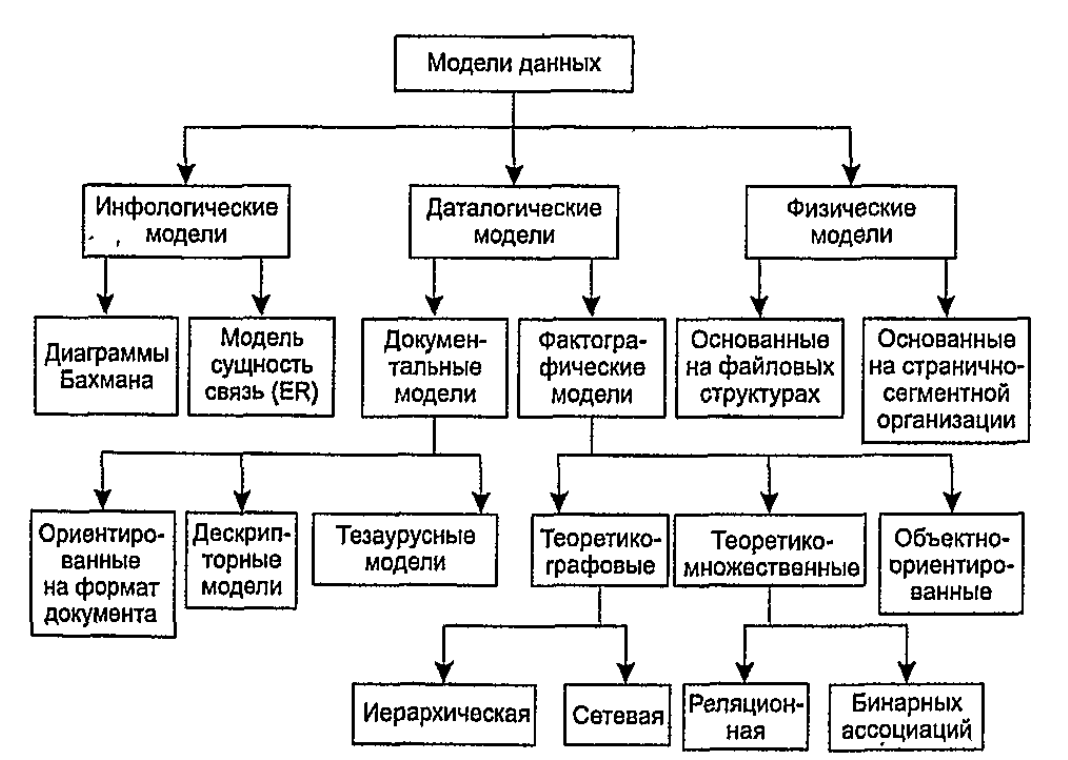
\includegraphics[width=16cm]{data_models}}
	\caption{Классификация моделей данных \cite{karpova02}.}
	\label{fig:data_models}
\end{figure}

\subsection{Типы хранилищ}

Выбор наиболее подходящего хранилища данных является ключевым для проекта. Хранилища данных делятся на разные группы в зависимости от методов структурирования данных и поддерживаемых операций. По используемой модели данных СУБД делятся на реляционные и нереляционные. По способу доступа к БД, СУБД делятся на файл-серверные, клиент-серверные и встраиваемые. Рассмотрим некоторые наиболее часто встречающиеся их типы.

\subsubsection{Реляционные базы данных}

Реляционные БД основаны на реляционной модели данных (РМД). РМД построена на таких разделах математики, как теория множеств и логика первого порядка. Реляционные БД являются наиболее широко распространенными, так как РМБ имеет под собой развитый математический аппарат.

Теоретической основой этой модели является теория отношений. Основной структурой данных в модели является отношение, именно поэтому модель получила название реляционной. Отношение имеет простую графическую интерпретацию, оно может быть представлено в виде таблицы.

Главным преимуществом РМД является простота представления и формирования баз данных. Управление данными в реляционных БД осуществляется с помощью декларативного языка запросов SQL (Structured Query Language), который основан на реляционной алгебре.

С другой стороны, РМД имеет следующие недостатки:

\begin{itemize}
	\item отсутствие механизма отображения связи типа «многие ко многим»;
	\item отсутствие возможности указания типов связей;
	\item отсутствие специальных механизмов навигации;
	\item потеря соответствия (impedance mismatch) – структуры данных, хранимые в памяти, и РМД не соответствуют друг другу, из-за чего, в частности, цена создания проекта с использованием реляционной модели данных увеличивается.
\end{itemize}

Перечисленные недостатки, с одной стороны, ведет к упрощению модели, что и сделало ее такой популярной, но с другой стороны, приводит к снижению скорости доступа к данным, увеличивает объем памяти, занимаемой БД. Кроме того, не каждую предметную область возможно представить в виде отношений – основного понятия РМД.

Примерами реляционных БД являются PostgreSQL, Oracle, Microsoft SQL Server.

\subsubsection{Нереляционные базы данных}

К нереляционным системам хранения данных относятся четыре типа систем: хранилище пар «ключ – значение», база данных документов (документоориентированная БД), семейство столбцов (БД столбцов) и база данных графов.

Хранилище пар «ключ-значение» представляет собой хэш-таблицу, то есть доступ к БД осуществляется через ключ. Обладает всеми преимуществами и недостатками этой структуры данных. Такие хранилища легко масштабируемы и имеют высокую производительность, однако не позволяют делать запросы сразу к нескольким хранилищам и не поддерживают запросы по значению. Хранилища пар «ключ – значение» чаще всего используются для хранения изображений и в качестве кэшей. Примеры хранилищ пар «ключ – значение»: Berkley DB, Redis.

Базы данных документов предназначены для хранения иерархических структур данных. В основе таких БД лежат хранилища, имеющие структуру дерева. Основной концепцией в таких БД является документ. Документы – это «самоописываемые иерархические структуры данных» \cite{nosql} (XML, JSON, BSON и т. д.). Примеры документоориентированных БД: MongoDB, CouchDB.

БД столбцов позволяют группировать значения в семейства столбцов, каждое из которых является ассоциативным массивом данных \cite{nosql}. Примеры: Apache HBase, Apache Cassandra.

Графовые БД предоставляют возможность хранить сущности и отношения между ними. Такие БД могут не справиться с большим объемом данным, если, например, необходимо изменить свойства всех сущностей, то есть выполнить операцию, затрагивающую весь граф. Примеры графовых БД: Neo4j, OrientDB.

В целом, можно отметить следующие преимущества нереляционных БД (NoSQL).

\begin{itemize}
	\item Возможность эффективно обрабатывать большие объемы данных на кластерах. Реляционные БД не предназначены для этого.
	\item Более удобный способ обмена данными, что повышает производительность разработки приложений.
	\item БД NoSQL работают без схемы, «позволяя свободно добавлять поля в базу данных без предварительного изменения структуры» \cite{nosql}. БД NoSQL не имеют ограничений на тип хранимых данных.
	\item NoSQL-базы лучше масштабируются (по сравнению с реляционными БД).
	\item Разработка NoSQL-базы требует меньше времени, чем разработка реляционной БД.
\end{itemize}

\subsubsection{Файл-серверные, клиент-серверные и встраиваемые БД}

В файл-серверных СУБД файлы данных расположены на файл-сервере, а СУБД расположена на каждой клиентской рабочей станции. Сейчас эта технология считается устаревшей и не рекомендуется к использованию. Примеры: Microsoft Access, Paradox.

В клиент-серверной СУБД и файлы данных и сама СУБД располагаются на сервере. Все запросы от клиентов выполняются централизованно. Такие СУБД предъявляют высокие требования к серверу. Примеры: PostgreSQL, Oracle, Microsoft SQL Server, MongoDB.

Встраиваемая БД является составной частью программного продукта. Она локально хранит данные конкретного приложения и не рассчитана на совместное использование. Примеры: SQLite, BerkleyDB, RocksDB, Firebird Embedded, Microsoft SQL Server Compact.

\subsection{Выбор типа хранилища}

Реляционная модель данных, с одной стороны, обладает простотой и наглядностью для пользователей-непрограммистов, а с другой -- серьезное теоретическое обоснование. Это определило большую популярность модели. Кроме того, развитие
формального аппарата представления и манипулирования данными в рамках реляционной модели сделали се наиболее перспективной для использования в системах представления знаний, что обеспечивает качественно иной подход к 
обработке данных в больших информационных системах.

По этим причинам в данной работе будет использоваться реляционная модель данных. С точки зрения доступа к БД, будет использоваться клиент-серверная СУБД, так как файл-серверные СУБД считаются устаревшими, а встраиваемые БД, хранящие данные локально, не подходят для централизованного хранения данных информационной системы ветеринарной клиники, которая будет иметь большое количество пользователей.

В качестве СУБД в данной работе будет использоваться PostgreSQL. PostgreSQL -- это мощная объектно-реляционная система баз данных с открытым исходным кодом, активная разработка которой насчитывает более 30 лет, что принесло ей прочную репутацию благодаря надежности, функциональной устойчивости и производительности. Кроме того, PostgreSQL имеет подробную официальную документацию и большое сообщество разработчиков.

\subsection{Диаграмма вариантов использования}

Исходя из анализа предментой области, необходимо выделить группы пользователей разабатываемой системы.

Диаграмма вариантов использования (диаграмма прецедентов или use-case диаграмма) описывает функциональное назначение системы. На диаграмме вариантов использования проектируемая система представляется в виде множества сущностей или актеров, взаимодействующих с системой с помощью вариантов использования.

Диаграмма вариантов использования представлена на рисунке \ref{fig:use_case}.

\begin{figure}[!h]
	\center{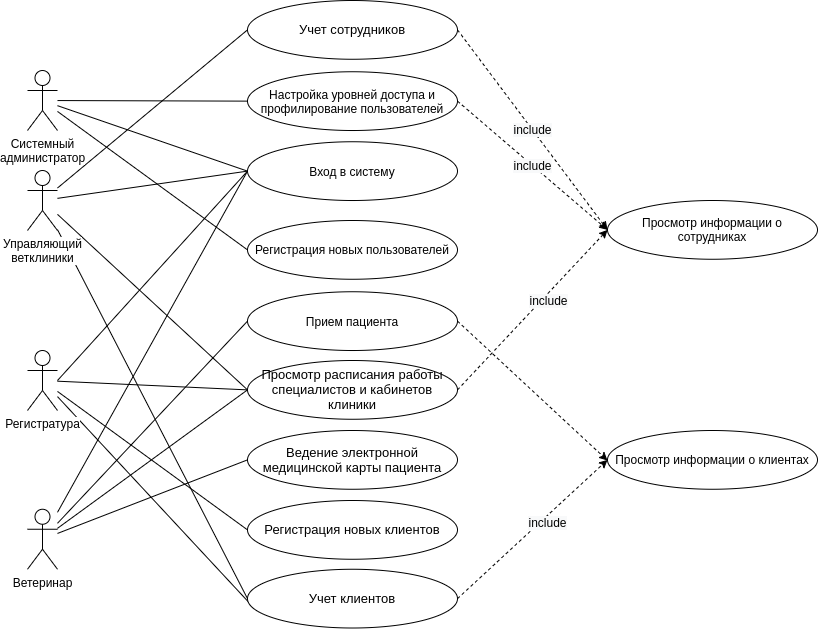
\includegraphics[width=16.5cm]{use_case}}
	\caption{Use-case диаграмма.}
	\label{fig:use_case}
\end{figure}

Выделяется четыре типа пользователей: системный администратор, управляющий ветеринарной клиники, сотрудник регистратуры и ветеринар. Пользователи взаимодействуют с системой и используют ее функциональные возможности для достижения определенных
целей. Для каждого типа пользователей предусмотрен свой набор возможностей.

Системный администратор:

\begin{itemize}
	\item настройка уровней доступа и профилирование пользователей;
	\item вход в систему;
	\item регистрация новых пользователей.
\end{itemize}

Управляющей ветеринарной клиники:

\begin{itemize}
	\item вход в систему;
	\item просмотр расписания работы специалистов и кабинетов клиники;
	\item учет клиентов.
\end{itemize}

Регистратура:

\begin{itemize}
	\item вход в систему;
	\item просмотр расписания работы специалистов и кабинетов клиники;
	\item регистрация новых клиентов;
	\item учет клиентов.
\end{itemize}

Ветеринар:

\begin{itemize}
	\item вход в систему;
	\item прием пациента;
	\item просмотр расписани работы специалистов и кабинетов клиники;
	\item ведение электронной медицинской карты пациента.
\end{itemize}

\subsection{Определение требований к структуре базы данных}

Для проектирования базы данных необходимо определить природу данных, с которыми придется работать.

Исходя из анализа предметной области, можно выделить следующие категории данных:

\begin{itemize}
	\item паспорт;
	\item адрес;
	\item клиент клиники;
	\item договор с клиентом;
	\item медицинская карта животного;
	\item чип животного;
	\item осмотр ветеринара;
	\item состояние животного;
	\item персонал клиники;
	\item должность в клинике;
	\item расписание;
	\item пользователи системы.
\end{itemize}

Каждая категория данных описывается информацией, описанной в таблице 1.

\begin{table}[!h]
	\caption{Категории данных и информация, которую они содержат.}
	\begin{center}
	%\tabcolsep=0.11cm
		\begin{tabular}{| c | c |}
	 	\hline
		Категория & Информация \\ \hline
	Паспорт &  Фамилия; имя; отчество; пол; \\
		& дата рождения; серия-номер паспорта; \\ & дата выдачи паспорта; национальность \\ \hline
	Адрес & страна; город; улица; \\
		& дом; квартира \\ \hline
    Клиент клиники & контакты; адрес; паспорт \\ \hline
	Договор с клиентом & номер договора; дата заключения; \\
		& дата последнего обновления; \\
		& клиент, с которым заключен договор; \\
		& дата истечения срока договора  \\ \hline
	Чип животного & номер чипа, дата имплантации; \\
		& страна имплантации; расположение чипа \\ \hline
	Медицинская карта животного & имя; порода; вид; пол; \\
		& отметка о кастрации; дата рождения; окрас; \\
		& особые приметы; дата постановки на учет; \\
		& чип; фотография; договор \\ \hline
	Осмотр ветеринара & врач; животное-пациент; \\
		& отметка об амбулаторном приеме; дата; \\
		& динамика состояния животного \\ 
		& со слов владельца; анамнез; \\ 
		& текущее состояние; диагноз; \\ 
		& рекоммендации; дата повторного осмотра \\ 
		& (если необходимо); назначения; \\
		& примечение; отметка о первичном осмотре \\ \hline
	Состояние животного & общее состояние; пульс; вес; \\
		& артериальное давление; температура; \\
		& скорость наполнения капилляров; \\
		& частота дыхательных движений \\ \hline
	Расписание & сотрудник; день недели; \\
		& время начала; время окончания; \\
		& кабинет \\ \hline
    Должность в клинике & название; зарплата \\ \hline
	Персонал клиники & паспорт; должность; уровень образования; \\
		& дата наема; дата увольнения \\ \hline
	Пользователи системы & сотрудник; логин; пароль; \\
		& уровень доступа. \\ \hline
	\end{tabular}
	\end{center}
\end{table}

\newpage
\subsection{Разработка логической модели данных}

Концептуальную схему предметной области позволяет описать ER-модель (модель сущность-связь). С её помощью можно выделить ключевые сущности и обозначить связи, которые могут устанавливаться между этими сущностями.

Диаграмма сущность-связь, описывающая выбранную предметную область, представлена на рисунке \ref{fig:er}.

\begin{figure}[!h]
	\center{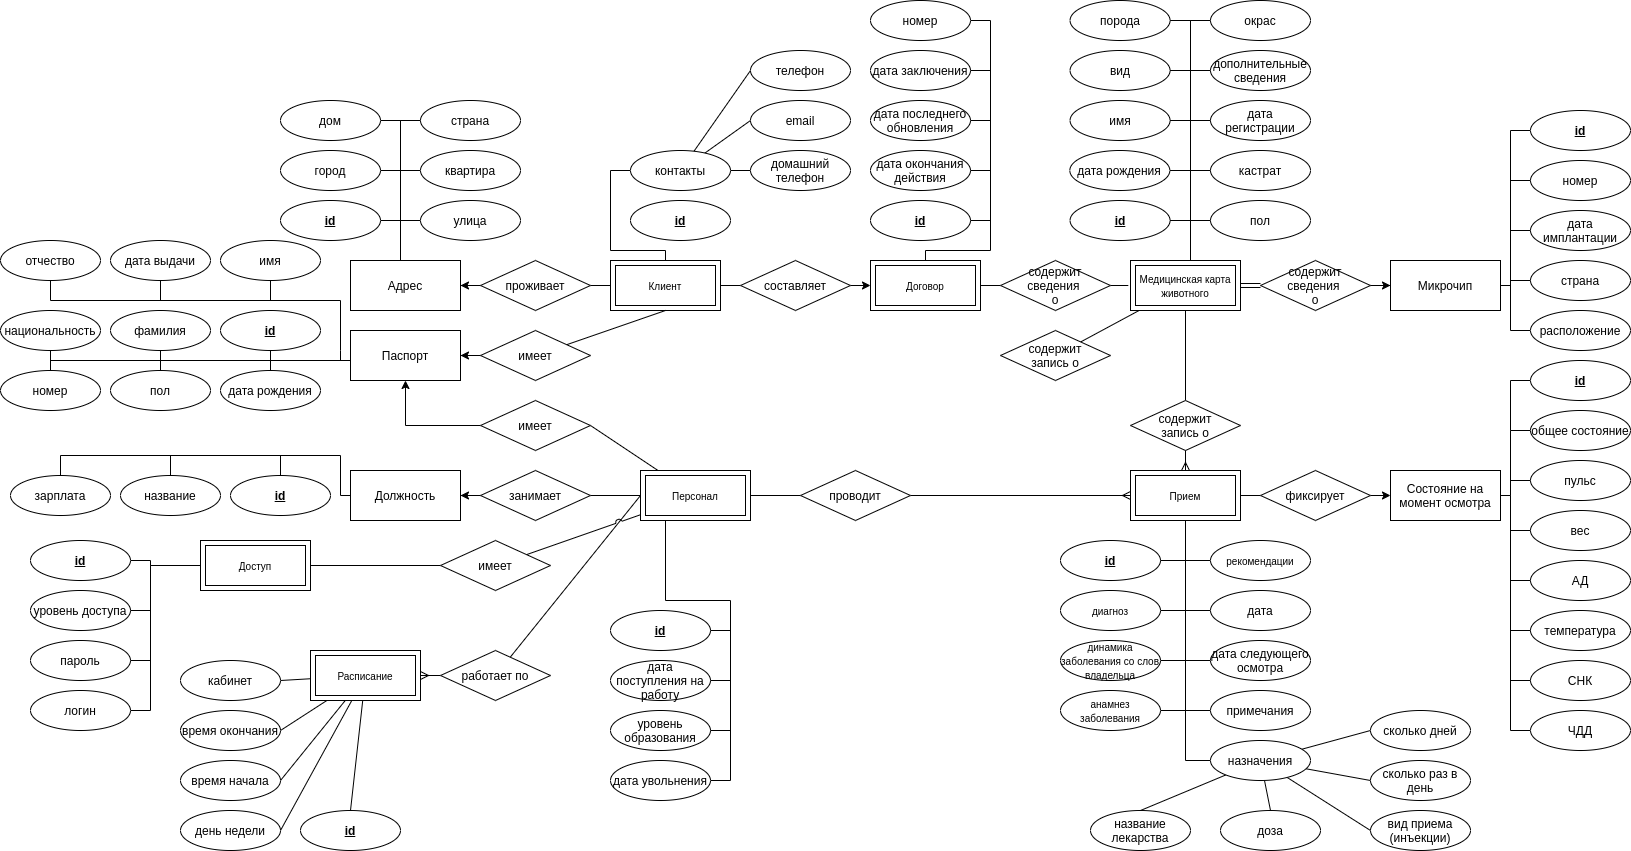
\includegraphics[width=23.5cm, angle=90]{er}}
	\caption{ER-диаграмма.}
	\label{fig:er}
\end{figure}

\newpage

\subsection{Архитектура приложения}

Архитектура программного обеспечения – совокупность важнейших решений об организации программной системы. Главной целью архитектуры ПО является упрощение разработки, развертывания и сопровождение программной системы.

В модели клиент-сервер роли определены следующим образом: сервер предоставляет ресурсы и службы одному или нескольким клиентам, которые обращаются к серверу за обслуживанием. Большинство серверов могут устанавливать отношение "один ко многим" с клиентами, что означает, что один сервер может предоставлять ресурсы нескольким клиентам одновременно. 

Когда клиент запрашивает соединение с сервером, сервер может либо принять, либо отклонить это соединение. Если соединение принято, сервер устанавливает и поддерживает соединение с клиентом по определенному протоколу . 

Часто клиенты и серверы взаимодействуют через компьютерную сеть на разных аппаратных средствах, но и клиент и сервер могут находиться в одной и той же системе. Хост сервера запускает одну или несколько серверных программ, которые совместно используют свои ресурсы с клиентами. 

Клиент не предоставляет общий доступ ни к одному из своих ресурсов, но запрашивает данные или службу у сервера. Поэтому клиенты инициируют сеансы связи с серверами, которые ожидают входящих запросов. Клиенту не знает о том, как работает сервер при выполнении запроса и доставке ответа. Клиент должен только понимать ответ, основанный на хорошо известном прикладном протоколе, т. е. содержание и форматирование данных для запрашиваемой службы. Клиенты и серверы обмениваются сообщениями в шаблоне обмена сообщениями запрос-ответ . Клиент отправляет запрос, а сервер возвращает ответ. 

Преимуществом модели взаимодействия клиент-сервер является то, что программный код клиентского приложения и серверного разделен. Кроме того, к машинам клиентов предъявляются пониженные требования, так как большая часть вычислительных операций будет производиться на сервере.

Схема взаимодействия по модели клиент-сервер представлена на рисунке \ref{fig:cli_ser}.

\begin{figure}[!h]
	\center{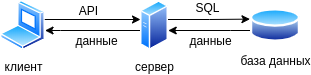
\includegraphics[width=10cm]{cli_ser}}
	\caption{Модель клиент-сервер.}
	\label{fig:cli_ser}
\end{figure}

\newpage
\textbf{Вывод из аналитического раздела}

Таким образом, в данном разделе был проведен анализ предметной области, формализация требований к программе, а также рассмотрены различные способы хранения данных в приложениях. Был произведен выбор типа хранилища и выбор СУБД. В качестве СУБД была выбрана PostgreSQL. Были выделены различные категории пользователей системы и построена диаграмма вариантов использования. Кроме того, была разработана логическая модель данных и построена ER-диаграмма предметной области.

\newpage
\section{Конструкторский раздел}

В данном разделе будет выполнено проектирование базы данных с учетом выбранной СУБД.

\subsection{Проектирование таблиц базы данных}

В предыдущем разделе были выделены ключевые сущности и обозначены связи между ними в рассматриваемой предметной области. В соответствии с выделенными выделенными сущностями, база данных должна содержать следующие таблицы.

\begin{itemize}
	\item Таблица адресов -- addresses.
	\item Таблица паспортов -- passports.
	\item Таблица клиентов -- clients.
	\item Таблица договоров -- contracts.
	\item Таблица микрочипов -- microchips.
	\item Таблица должностей -- position.
	\item Таблица состояний животного -- animal\_states.
	\item Таблица медицинских карт животных -- animal\_medical\_records.
	\item Таблица персонала -- staff.
	\item Таблица осмотров -- visits.
	\item Таблица пользователей системы -- access.
	\item Таблица расписания -- schedule.
\end{itemize}

Рассмотрим подробнее каждую из таблиц. Названия столбцов, их тип, ограничения и пояснения к столбцам каждой из 12 перечисленных таблиц БД представлены в таблицах 2-13. Типы выбраны в соответствии с теми тем, какие типы предоставляет СУБД PostgreSQL.

\newpage
\begin{table}[!h]
	\caption{Столбцы таблицы адресов addresses.}
	\begin{center}
	%\tabcolsep=0.11cm
		\begin{tabular}{| c | c | c | c |}
	 	\hline
		Название & Тип & Ограничения & Пояснение \\ \hline
		addr\_id & SERIAL & NOT NULL, & Идентификатор адреса \\ 
		& & PRIMARY KEY & \\ \hline
		country & VARCHAR(64) & NOT NULL & Наззвание страны \\ \hline
		city & VARCHAR(255) & NOT NULL & Название города \\ \hline
		street & VARCHAR(255) & NOT NULL & Название улицы \\ \hline
		house & VARCHAR(10) & NOT NULL & Номер дома \\ \hline
		flat & VARCHAR(10) & - & Номер квартиры \\ 
		& & & (если есть) \\ \hline
	\end{tabular}
	\end{center}
\end{table}

\begin{table}[!h]
	\caption{Столбцы таблицы паспортов passports.}
	\begin{center}
	%\tabcolsep=0.11cm
		\begin{tabular}{| c | c | c | c |}
	 	\hline
		Название & Тип & Ограничения & Пояснение \\ \hline
		pass\_id & SERIAL & NOT NULL, & Идентификатор паспорта \\ 
		& & PRIMARY KEY & \\ \hline
		surname & VARCHAR(64) & NOT NULL & Фамилия \\ \hline
		name & VARCHAR(64) & NOT NULL & Имя \\ \hline
		patronymic & VARCHAR(64) & - & Отчество \\
		 &  &  & (если есть) \\ \hline
		sex & sex\_type & NOT NULL & Пол \\ 
		 &  &  & (необходимо определить \\ 
		 &  &  & пользовательский тип) \\ \hline
		birth & DATE & NOT NULL & Дата рождения \\ \hline
		num & VARCHAR(10) & NOT NULL & Серия-номер паспорта \\ \hline
		issue\_date & DATE & NOT NULL & Дата выдачи паспорта \\ \hline
		nationality & VARCHAR(128) & - & Национальность \\
		 &  &  & (если указана) \\ \hline
	\end{tabular}
	\end{center}
\end{table}

\newpage
\begin{table}[!h]
	\caption{Столбцы таблицы клиентов clients.}
	\begin{center}
	%\tabcolsep=0.11cm
		\begin{tabular}{| c | c | c | c |}
	 	\hline
		Название & Тип & Ограничения & Пояснение \\ \hline
		cli\_id & SERIAL & NOT NULL &  \\
		 &  & PRIMARY KEY & Идентификатор клиента \\ \hline
		contacts & JSON & NOT NULL & Контакты \\ \hline
		address & INT & NOT NULL & Идентификатор адреса клиента \\ \hline
		passport & INT & NOT NULL & Идентификатор паспорта клиента \\ \hline
	\end{tabular}
	\end{center}
\end{table}

\begin{table}[!h]
	\caption{Столбцы таблицы договоров contracts.}
	\begin{center}
	%\tabcolsep=0.11cm
		\begin{tabular}{| c | c | c | c |}
	 	\hline
		Название & Тип & Ограничения & Пояснение \\ \hline
		contr\_id & SERIAL & NOT NULL & Идентификатор договора \\
		 &  & PRIMARY KEY &  \\ \hline
		code & VARCHAR(20) & NOT NULL & Номер договора \\ \hline
		conclusion\_date & DATE & NOT NULL & Дата заключения \\  &  &  & договора \\ \hline
		last\_update\_date & DATE & NOT NULL &  \\ \hline
		owner & INT & NOT NULL & Дата последнего \\ 
		 &  &  & обновления договора \\
		 &  &  & (повторное заключение) \\ \hline
		valid\_until & DATE & NOT NULL & Дата истечения \\
		 &  &  & договора \\ \hline
	\end{tabular}
	\end{center}
\end{table}

\begin{table}[!h]
	\caption{Столбцы таблицы микрочипов microchips.}
	\begin{center}
	%\tabcolsep=0.11cm
		\begin{tabular}{| c | c | c | c |}
	 	\hline
		Название & Тип & Ограничения & Пояснение \\ \hline
		chip\_id & SERIAL & NOT NULL &  \\
		 &  & PRIMARY KEY & Идентификатор чипа \\ \hline
		chip\_num & VARCHAR(15) & NOT NULL & Номер чипа \\ \hline
		impl\_date & DATE & NOT NULL & Дата имплантации \\ \hline
		country & VARCHAR(3) & NOT NULL & Трехбуквенный код страны, \\
		&  &  & где чип был имплантирован \\ \hline
		location & TEXT & NOT NULL & Расположение чипа \\ \hline
	\end{tabular}
	\end{center}
\end{table}

\newpage
\begin{table}[!h]
	\caption{Столбцы таблицы должностей position.}
	\begin{center}
	%\tabcolsep=0.11cm
		\begin{tabular}{| c | c | c | c |}
	 	\hline
		Название & Тип & Ограничения & Пояснение \\ \hline
		pos\_id & SERIAL & NOT NULL & Идентификатор должности \\
		 &  & PRIMARY KEY &  \\ \hline
		title & VARCHAR(256) & NOT NULL & Название должности \\ \hline
		salary & INT & NOT NULL & Заработная плата \\
		salary & INT & NOT NULL & (в рублях) \\ \hline
	\end{tabular}
	\end{center}
\end{table}

\begin{table}[!h]
	\caption{Столбцы таблицы состояний животного animal\_states.}
	\begin{center}
	%\tabcolsep=0.11cm
		\begin{tabular}{| c | c | c | c |}
	 	\hline
		Название & Тип & Ограничения & Пояснение \\ \hline
		state\_id & SERIAL & NOT NULL & Идентификатор состояния \\
		 &  & PRIMARY KEY &  \\ \hline
		general & general\_type & NOT NULL & Общее состояние (необходим \\
		 &  &  & пользовательский тип) \\ \hline
		pulse & INT & NOT NULL & Пульс \\ \hline
		weight & REAL & NOT NULL & Вес в кг \\ \hline
		ap & VARCHAR(10) & NOT NULL & Артериальное давление \\ \hline
		temperature & REAL & NOT NULL & Температура тела в  \\
		 &  &  & градусах по Цельсию  \\ \hline
		cfr & INT & NOT NULL & Скорость наполнения \\
		 &  &  & каппиляров (в секундах) \\ \hline
		resp\_rate & INT & NOT NULL & Частота дыхательных \\
		 &  &  & движений \\ \hline
	\end{tabular}
	\end{center}
\end{table}

\newpage
\begin{table}[!h]
	\caption{Столбцы таблицы медицинских карт animal\_medical\_records.}
	\begin{center}
	%\tabcolsep=0.11cm
		\begin{tabular}{| c | c | c | c |}
	 	\hline
		Название & Тип & Ограничения & Пояснение \\ \hline
		anim\_id & SERIAL & NOT NULL & Идентификатор \\
		 &  & PRIMARY KEY & карты \\ \hline
		name & VARCHAR(64) & NOT NULL & Имя животного \\ \hline
		breed & TEXT & NOT NULL & Порода \\ \hline
		species & TEXT & NOT NULL & вид \\ \hline
		sex & sex\_type & NOT NULL & Пол \\ \hline
		castrated & BOOLEAN & NOT NULL & Отметка о \\
		 &  & DEFAULT('f') & стерилизации \\ \hline
		birth & DATE & NOT NULL & Дата рождения \\ \hline
		other\_data & TEXT & NOT NULL & Дополнительные \\
		 &  &  & сведения \\ \hline
		color & TEXT & NOT NULL & Окрас \\ \hline
		special\_signs & TEXT & NOT NULL & Особые приметы \\ \hline
		registr\_date & DATE & NOT NULL & Дата регистрации \\
		 &  &  & в клинике \\ \hline
		chip\_id & INT & NOT NULL & Идентификатор \\
		 & &  & чипа \\ \hline
		contract & INT & NOT NULL & Идентификатор \\ \hline
		 &  & & договора \\ \hline
		rel\_path\_to\_photo & VARCHAR(255) & NOT NULL & Относительный путь \\
		 &  &  & до фотографии \\ \hline
	\end{tabular}
	\end{center}
\end{table}

\begin{table}[!h]
	\caption{Столбцы таблицы персонала staff.}
	\begin{center}
	%\tabcolsep=0.11cm
		\begin{tabular}{| c | c | c | c |}
	 	\hline
		Название & Тип & Ограничения & Пояснение \\ \hline
		staff\_id & SERIAL & NOT NULL & Идентификатор сотрудника \\
		 & & PRIMARY KEY &  \\ \hline
		passport & INT & NOT NULL & Идентификатор паспорта \\ \hline
		position & INT & NOT NULL & Идентификатор должности \\ \hline
		edu\_level & edu\_level\_type & NOT NULL & Уровень образования \\ \hline
		fire\_date & DATE & - & Дата увольнения \\
		 &  &  & (если уволен) \\ \hline
		employ\_date & DATE & NOT NULL & Дата найма \\ \hline
	\end{tabular}
	\end{center}
\end{table}

\newpage
\begin{table}[!h]
	\caption{Столбцы таблицы осмотров visits.}
	\begin{center}
	%\tabcolsep=0.11cm
		\begin{tabular}{| c | c | c | c |}
	 	\hline
		Название & Тип & Ограничения & Пояснение \\ \hline
		vis\_id & SERIAL & NOT NULL & Идентификатор \\ 
		 &  & PRIMARY KEY & осмотра \\ \hline
		doctor & INT & NOT NULL & Идентификатор \\
		 &  &   & ветеринара \\ \hline
		animal & INT & NOT NULL & Идентификатор \\
		 &  &   & карты животного \\ \hline
		visit\_date & DATE & NOT NULL & Дата осмотра \\ \hline
		owner\_dynamics & owner\_dynamics\_type & NOT NULL & Динамика \\
		&  &  & состояния со \\
		 &  &  & слов владельца \\ \hline
		history\_disease & TEXT & NOT NULL & Анамнез \\ \hline
		cur\_state & INT & NOT NULL & Идентификатор \\
		 &  & & текущего \\ 
		 &  &  & состояния \\ \hline
		diagnosis & TEXT & NOT NULL & Диагноз \\ \hline
		recommendations & TEXT & NOT NULL & Рекоммендации \\ \hline
		next\_visit & DATE & - & Дата \\
		 &  &  & повторного \\
		 &  &  & осмотра \\ \hline
		prescribings & JSON & - & Назначения \\ \hline
		note & TEXT & - & Примечания \\ \hline
	\end{tabular}
	\end{center}
\end{table}

\newpage
\begin{table}[!h]
	\caption{Столбцы таблицы пользователей системы access.}
	\begin{center}
	%\tabcolsep=0.11cm
		\begin{tabular}{| c | c | c | c |}
	 	\hline
		Название & Тип & Ограничения & Пояснение \\ \hline
		acc\_id & SERIAL & NOT NULL & Идентификатор \\
		 &  & PRIMARY KEY & аккаунта \\ \hline
		employee & INT & NOT NULL & Идентификатор \\
		& &  & сотрудника \\ \hline
		login & VARCHAR(64) & NOT NULL & Логин \\ \hline
		password & BYTEA & NOT NULL & Пароль \\ \hline
		access\_level & access\_level\_type & NOT NULL & Уровень доступа \\ 
		& &  & (пользовательский \\ 
		& &  & тип) \\ \hline
	\end{tabular}
	\end{center}
\end{table}

\begin{table}[!h]
	\caption{Столбцы таблицы расписания schedule.}
	\begin{center}
	%\tabcolsep=0.11cm
		\begin{tabular}{| c | c | c | c |}
	 	\hline
		Название & Тип & Ограничения & Пояснение \\ \hline
		shed\_id & SERIAL & NOT NULL &  Идентификатор \\
		&  & PRIMARY KEY & расписания \\ \hline
		employee\_id & INT & NOT NULL & Идентификатор \\
		 &  &  & сотрудника \\ \hline
		day\_of\_week & day\_of\_week\_type & NOT NULL & День недели  \\ \hline
		start & TIMESTAMP & NOT NULL & Время начала \\ 
		 &  &  & рабочего дня \\ \hline
		end & TIMESTAMP & NOT NULL & Время окончания \\
		 &  &  & рабочего дня \\ \hline
		cabinet & VARCHAR(10) & - & кабинет \\
		&  & & (если есть) \\ \hline
	\end{tabular}
	\end{center}
\end{table}

\subsection{Сценарий создания базы данных}

Сцернарий создания базы данных приведен в листинге \ref{db_create}.

\begin{lstlisting}[label=db_create,caption=\text{Сценарий создания БД.}]
#!/bin/bash
# Required package: jq
	
ps_user=`jq '.username' dist.conf | tr -d \"`
db_name=`jq '.db_name' dist.conf | tr -d \"`
pwd=`pwd`
	
createdb -U $ps_user $db_name

cd ../scripts/update
	
files=`ls -r update_*.sql | sort`
for VAR in $files
do
	psql -U $ps_user -d $db_name -f $VAR 
done
	
cd $pwd
\end{lstlisting}

Конфигурационный файл для этого сценария приведен в листинге \ref{config}.

\begin{lstlisting}[label=config,caption=\text{Конфигурационный файл.}]
{
	"username" : "postgres",
	"db_name" : "vet"
}
\end{lstlisting}

Сценарий первой ревизии БД представлен в листинге \ref{first_rev}.

\begin{lstlisting}[label=first_rev,caption=\text{Первая ревизия.}]
---- first revision

\i ../install/create_passport.sql
\i ../install/create_access.sql
\i ../install/create_addresses.sql
\i ../install/create_animal_medical_records.sql
\i ../install/create_animal_states.sql
\i ../install/create_client.sql
\i ../install/create_contract.sql
\i ../install/create_microchips.sql
\i ../install/create_position.sql
\i ../install/create_schedule.sql
\i ../install/create_staff.sql
\i ../install/create_visits.sql
\end{lstlisting}

\subsection{Определение пользовательских типов в БД}

Как видно из предыдущего подраздела, для создания таблиц БД необходимо определить несколько пользовательских типов. Сценарий создания пользовательких типов приведен в листинге \ref{types}.

\begin{lstlisting}[label=types,caption=\text{Определение прользовательских типов.}]
CREATE TYPE access_level_type AS ENUM('admin', 'main', 'registry', 'vet');

CREATE TYPE general_type AS ENUM('middle', 'good', 'bad');

CREATE TYPE sex_type AS ENUM ('m', 'f', 'other');

CREATE TYPE day_of_week_type AS ENUM('Sun', 'Mon', 'Tue', 'Wed', 'Thu', 'Fri', 'Sat');

CREATE TYPE edu_level_type AS ENUM('resident', 'middle', 'postgraduate', 'specialist', 'bachelor');

CREATE TYPE owner_dynamics_type AS ENUM('stably', 'worse', 'better');
\end{lstlisting}

\subsection{Сценарий создания таблиц БД}

Сценарий создания таблиц БД представлен в листинге \ref{tables}.

\begin{lstlisting}[label=tables,caption=\text{Создание таблиц БД.}]
CREATE TABLE access(
	acc_id SERIAL NOT NULL PRIMARY KEY,
	employee INT NOT NULL,
	login VARCHAR(64) NOT NULL,
	password BYTEA NOT NULL,
	access_level access_level_type NOT NULL
);

CREATE TABLE addresses(
	addr_id SERIAL NOT NULL PRIMARY KEY,
	country VARCHAR(64) NOT NULL,
	city VARCHAR(255) NOT NULL,
	street VARCHAR(255) NOT NULL,
	house VARCHAR(10) NOT NULL,
	flat VARCHAR(10)
);

CREATE TABLE animals_medical_records(
    anim_id SERIAL NOT NULL PRIMARY KEY,
    name VARCHAR(64) NOT NULL,
    breed TEXT NOT NULL,
    species TEXT NOT NULL,
    sex sex_type NOT NULL,
    castrated BOOLEAN NOT NULL DEFAULT('f'),
    birth DATE NOT NULL,
    other_data TEXT NOT NULL,
    color TEXT NOT NULL,
    special_signs TEXT NOT NULL,
    registr_date DATE NOT NULL,
    chip_id INT NOT NULL,
    contract INT NOT NULL,
    rel_path_to_photo VARCHAR(255) NOT NULL
);

CREATE TABLE animal_states(
    state_id SERIAL NOT NULL PRIMARY KEY,
    general general_type NOT NULL,
    pulse INT NOT NULL,
    weight REAL NOT NULL,
    ap VARCHAR(10) NOT NULL,
    temperature REAL NOT NULL,
    cfr INT NOT NULL,
    resp_rate INT NOT NULL
);

CREATE TABLE clients(
	cli_id SERIAL NOT NULL PRIMARY KEY,
	contacts JSON NOT NULL,
	address INT NOT NULL,
	passport INT NOT NULL
);

CREATE TABLE contract(
	contr_id SERIAL NOT NULL PRIMARY KEY,
	code VARCHAR(20) NOT NULL,
	conclusion_date DATE NOT NULL,
	last_update_date DATE NOT NULL,
	"owner" INT NOT NULL,
	valid_until DATE NOT NULL
);

CREATE TABLE microchips(
    chip_id SERIAL NOT NULL PRIMARY KEY,
    chip_num VARCHAR(15) NOT NULL,
    impl_date DATE NOT NULL,
    country VARCHAR(3) NOT NULL,
    location TEXT NOT NULL
);

CREATE TABLE passports(
	pass_id SERIAL NOT NULL PRIMARY KEY,
	surname VARCHAR(64) NOT NULL,
	name VARCHAR(64) NOT NULL,
	patronymic VARCHAR(64),
	sex sex_type NOT NULL,
	birth DATE NOT NULL,
	num VARCHAR(10) NOT NULL,
	issue_date DATE NOT NULL,
	nationality VARCHAR(128)
);

CREATE TABLE position(
	pos_id SERIAL NOT NULL PRIMARY KEY,
	title VARCHAR(256) NOT NULL,
	salary INT NOT NULL
);

CREATE TABLE schedule(
    shed_id SERIAL NOT NULL PRIMARY KEY,
    employee_id INT NOT NULL,
    day_of_week day_of_week_type NOT NULL,
    "start" TIME NOT NULL,
    "end" TIME NOT NULL,
    cabinet VARCHAR(10)
);

CREATE TABLE staff(
	staff_id SERIAL NOT NULL PRIMARY KEY,
	passport INT NOT NULL,
	position INT NOT NULL,
	edu_level edu_level_type NOT NULL,
	fire_date DATE,
	employ_date DATE NOT NULL
);

CREATE TABLE visits(
    vis_id SERIAL NOT NULL PRIMARY KEY,
    doctor INT NOT NULL,
    animal INT NOT NULL,
    visit_date DATE NOT NULL,
    owner_dynamics owner_dynamics_type NOT NULL,
    history_disease TEXT NOT NULL,
    cur_state INT NOT NULL,
    diagnosis TEXT NOT NULL,
    recommendations TEXT NOT NULL,
    next_visit DATE,
    prescribings JSON,
    note TEXT
);
\end{lstlisting}

Вторая ревизия базы данных -- создание ограничений в таблицах -- представлена в листинге \ref{constraints}.

\begin{lstlisting}[label=constraints,caption=\text{Создание органичений.}]
---- add constraint

ALTER TABLE clients ADD CONSTRAINT addr_client_fk 
	FOREIGN KEY (address) REFERENCES addresses(addr_id) 
	ON DELETE CASCADE;
	
ALTER TABLE clients ADD CONSTRAINT pass_client_fk 
	FOREIGN KEY (passport) REFERENCES passports(pass_id) 
	ON DELETE CASCADE;
	
ALTER TABLE staff ADD CONSTRAINT pass_staff_fk 
	FOREIGN KEY (passport) REFERENCES passports(pass_id) 
	ON DELETE CASCADE;
	
ALTER TABLE staff ADD CONSTRAINT pos_staff_fk 
	FOREIGN KEY (position) REFERENCES position(pos_id) 
	ON DELETE CASCADE;
	
ALTER TABLE access ADD CONSTRAINT stf_empl_fk 
	FOREIGN KEY (employee) REFERENCES staff(staff_id) 
	ON DELETE CASCADE;
	
ALTER TABLE contract ADD CONSTRAINT own_cntr_fk 
	FOREIGN KEY ("owner") REFERENCES clients(cli_id) 
	ON DELETE CASCADE;
	
ALTER TABLE schedule ADD CONSTRAINT empl_schdl_fk 
	FOREIGN KEY (employee_id) REFERENCES staff(staff_id) 
	ON DELETE CASCADE;
	
ALTER TABLE animals_medical_records ADD CONSTRAINT anmr_ctrc_fk 
	FOREIGN KEY (contract) REFERENCES contract(contr_id) 
	ON DELETE CASCADE;
	
ALTER TABLE animals_medical_records ADD CONSTRAINT anmr_mchp_fk 
	FOREIGN KEY (chip_id) REFERENCES microchips(chip_id) 
	ON DELETE CASCADE;
	
ALTER TABLE visits ADD CONSTRAINT vis_schdl_fk 
	FOREIGN KEY (doctor) REFERENCES staff(staff_id) 
	ON DELETE CASCADE;
	
ALTER TABLE visits ADD CONSTRAINT vis_anmr_fk 
	FOREIGN KEY (animal) REFERENCES animals_medical_records(anim_id) 
	ON DELETE CASCADE;
	
ALTER TABLE visits ADD CONSTRAINT vsts_asts_fk 
	FOREIGN KEY (cur_state) REFERENCES animal_states(state_id) 
	ON DELETE CASCADE;
	
ALTER TABLE passports ADD CONSTRAINT unique_pass_num UNIQUE(num);
	
ALTER TABLE microchips ADD CONSTRAINT unique_mchip_num UNIQUE(chip_num);
\end{lstlisting}

\subsection{Диаграмма базы данных}

Диаграмма базы данных представлена на рисунке \ref{fig:db_dia}.


\begin{figure}[!h]
	\center{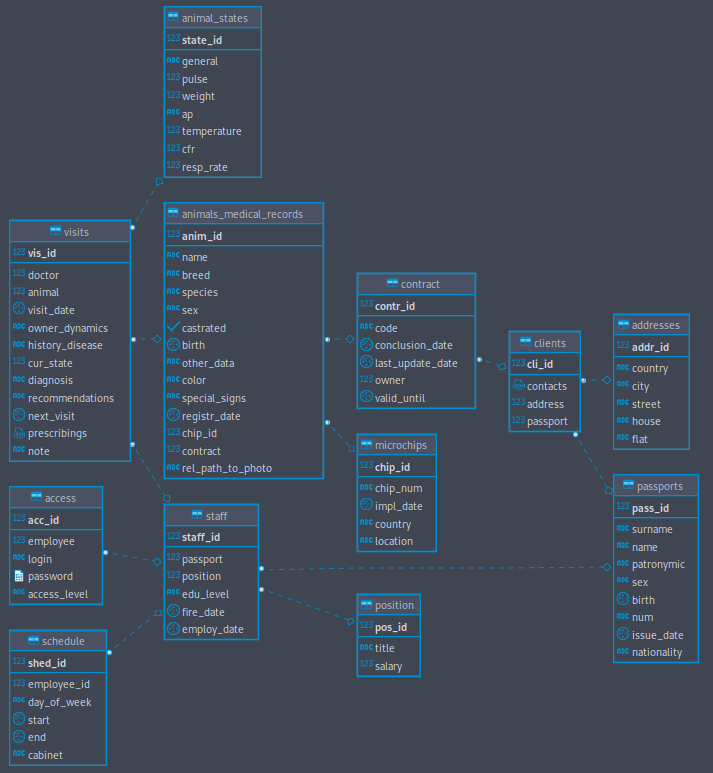
\includegraphics[width=16.5cm]{db_dia}}
	\caption{Диаграмма базы данных.}
	\label{fig:db_dia}
\end{figure}

\subsection{Паттерны проектирования}

В настоящее время при создании приложений с графическими пользовательскими интерфейсами применяются специальные паттерны проектирования, позволяющие синхронизировать разные функциональные области программного продукта между собой. Такие паттерны предназначены для уменьшения трудозатрат (и, как следствие, финансовых затрат) на разработку сложного программного обеспечения.

Фундаментальным паттерном, который нашел применение во многих технологиях и дал развитие новым, является паттерн MVC ( Model-View-Controller). Этот паттерн позволяет отделить графический пользовательский интерфейс от логики программирования. Это позволяет разрабатывать логику независимо от GUI.

MVC состоит из трех компонент: View (представление, пользовательский интерфейс), Model (модель, бизнес логика) и Controller (контроллер, содержит логику на изменение модели при определенных действиях пользователя, реализует Use Case). Основная идея этого паттерна в том, что и контроллер и представление зависят от модели, но модель никак не зависит от этих двух компонент. Это позволяет разрабатывать и тестировать модель, ничего не зная о представлениях и контроллерах. Контроллер так же ничего не должен знать о представлении (в иделе, а на практике это не всегда так).

Модель предоставляет данные и методы работы с ними: запросы в базу данных, проверка на корректность. Модель не зависит от представления (не знает как данные визуализировать) и контроллера (не имеет точек взаимодействия с пользователем), просто предоставляя доступ к данным и управлению ими.

Модель строится таким образом, чтобы отвечать на запросы, изменяя своё состояние. Модель, за счёт независимости от визуального представления, может иметь несколько различных представлений.

Представление отвечает за получение необходимых данных из модели и отправляет их пользователю. Представление не обрабатывает введённые данные пользователя.

Контроллер обеспечивает связь между пользователем и системой, контролирует и направляет данные от пользователя к системе и наоборот. Контроллер использует модель и представление для реализации необходимого действия. 

\subsection{Архитектура REST}

REST (Representational state transfer) – это стиль архитектуры программного обеспечения для распределенных систем, таких как World Wide Web. REST является очень простым интерфейсом управления информацией без использования каких-то дополнительных внутренних прослоек. Каждая единица информации однозначно определяется глобальным идентификатором, таким как URL. Каждая URL в свою очередь имеет строго заданный формат. 

REST представляет собой согласованный набор ограничений, учитываемых при проектировании распределённой гипермедиа-системы.

Для каждой единицы информации (info) определяется 5 действий.

\begin{itemize}
	\item GET /info/(Index) – получает список всех объектов. Как правило, это упрощенный список, то есть содержащий только поля идентификатора и названия объекта, без остальных данных.
	\item GET /info/{id}(View) – получает полную информацию об объекте.
	\item PUT /info/илиPOST /info/(Create) – создает новый объект. Данные передаются в теле запроса без применения кодирования, даже urlencode.
	\item POST /info/{id}илиPUT /info/{id}(Edit) – изменяет данные с идентификатором {id}, возможно, заменяетих. Данные также передаются в теле запроса, но, в отличие от PUT, здесь есть некоторый нюанс. Дело в том, что POST-запрос подразумевает наличие urldecoded-post-data. Т.е. если не применять кодирования – это нарушение стандарта.
	\item DELETE /info/{id}(Delete) – удаляет данные с идентификатором {id}.
\end{itemize}

Существует шесть обязательных ограничений для построения распределённых REST-приложений.

\begin{enumerate}
	\item Модель клиент-сервер. Необходимо привести архитектуру приложения к модели клиент-сервер.
	\item Отсутствие состояния. В период между запросами клиента никакая информация о состоянии клиента на сервере не хранится. То есть при выполнении запроса клиент передает серверу всю необходимую для выполнения запроса информацию.
	\item Кэширование. Клиенты могут выполнять кэширование ответов сервера.
	\item Единообразие интерфейса. К унифицированным интерфейсам предъявляются следующие требования.
	\begin{itemize}
		\item Идентификация ресурсов. Все ресурсы идентифицируются в запросах.
		\item Манипуляция ресурсами через представление. 
		\item «Самоописываемые» сообщения. Каждое сообщение содержит достаточно информации, чтобы понять, каким образом его обрабатывать.
	\end{itemize}
	\item Слои. Клиент обычно не способен точно определить, взаимодействует он напрямую с сервером или же с промежуточным узлом, в связи с иерархической структурой сетей.
	\item Код по требованию. REST может позволить расширить функциональность клиента за счёт загрузки кода с сервера в виде апплетов или сценариев.
\end{enumerate}

\textbf{Вывод из конструкторского раздела}

Таким образом, в данном разделе была спроектирована база данных, были разработаны сценарии создания базы данных и приведена ее окончательная схема. Кроме того, был рассмотрен фундаментальный паттерн проектирования, который будет применяться в настоящей работе.

\newpage
\section{Технологический раздел}

В данном разделе будут рассмотрены средства реализации проекта, приведены листинги и интерфейс приложения.

\subsection{Выбор языка программирования и среды разработки}

Выберем языки программирования и фреймворки для написания серверной и клиентской частей приложения.

\subsubsection{Серверная часть}

В качетсве языка программирования для написания серверной части был выбран Python и библиотека Flask. Flask -- это легковесный фреймворк для создания веб-приложений на Python, использующий набор инструментов Werkzeug.

Flask можно считать лучшим веб-фреймворком для создания веб-приложений на Python по следующим причинам.

\begin{itemize}
	\item Flask практически не зависит от внешних библиотек.
	\item Flask легок для понимания, имеет простую структуру и интуитивно понятный синтаксис.
	\item Flask позволяет довольно быстро создать веб-приложение, в отличие, от, например, Django.
	\item Гибкость. Большую часть инструментов фреймворка можно редактировать под свои нужды.
	\item Наличие хороших инструментов для тестирования, встроенного сервера разработки.
\end{itemize}

Недостатком Flask является то, что он не поддерживает асинхронность и обрабатывает все запросы в один поток. Однако в рамках учебного проекта этот недостаток незначителен.

\textbf{Взаимодействие с базой данных в Python}

Для взаимодействия с базой данных в Python был выбран модуль pyodbc. pyodbc - это модуль Python с открытым исходным кодом, который упрощает доступ к базам данных ODBC. Он реализует спецификацию DB API 2.0. Python DB API определяет независимый от базы данных интерфейс для данных, хранящихся в реляционных базах данных.

\subsubsection{Клиентская часть}

Для разработки клиентского приложения был выбран язык C++ и фреймворк Qt. Главным преимуществом Qt является платформонезависимость. Qt предоставляет под­
держку большого числа операционных систем: Microsoft Windows, Мае OS Х, Linux,
FreeBSD и других клонов UNIX с Х 11, а также и для мобильных операционных систем IOS,
Android, Windows Phone, Windows RT и BlackBeгry. 

Qt использует интерфейс API низкого уровня, что позволяет кроссплатформенным приложениям работать не менее эффективно, чем приложениям, разработанным под конкретную платформу. Qt не только является средством создания интерфейса пользователя, но и предоставляет полный инструментарий для программирования, который включает в себя поддержку двух- и трехмерной графики, возможность интернационализации, использование форматов JSON и XML,  STL-совместимую библиотеку контейнеров, поддержку стандартных протоколов ввода/вывода, классы для работы с сетью, поддержку программирования баз данных, включая Oracle, Microsoft SQL Server, IВМ 082, MySQL, SQLite, Sybase, PostgreSQL и т.д. 

Qt является полностью объектно-ориентированной библиотекой, использующей новую концепцию межобъектных коммуникаций <<сигналы и слоты>>. Qt имеет подробную официальную документацию, что значительно упрощает ее изучение.

\textbf{Сетевое взаимодействие на стороне клиента}

Первоначально для отправки сетевых запросов и получения ответов использовался класс QNetworkAccessManager. Однако он приводил к крахам всего приложения, поэтому был написанный собственный класс NetworkFetcher для общения с сервером. Он был написан с использованием библиотеки libcurl. 

libcurl -- это бесплатная и простая в использовании библиотека для передачи URL-адресов на стороне клиента. libcurl является легко переносимой библиотекой, она одинаково работает на многих платформах. Кроме того, libcurl является хорошо документированной.

Заголовочный файл класса NetworkFetcher приведен в листинге \ref{net_h}, а реализация -- в листинге \ref{net_cpp}.

\begin{lstlisting}[label=net_h,caption=\text{network\_fetcher.h.}]
#pragma once

#include <memory>
#include <curl/curl.h>
#include <QUrl>
#include <QVector>
#include <QNetworkRequest>
	
class Multipart final
{
	void addPart(const QString&, const QByteArray&);
	void addFilePart(const QString&, const QString&);

private:
	using Part = std::tuple<QByteArray, bool, QString>;
	QMap<QString, Part> parts;
};

class NetworkFetcher final
{
	struct RequestInfo;
	struct Info;
public:
	using Header = std::tuple<QString, QByteArray>;
	using AuthData = std::tuple<QString, QString>;
	using Response = std::tuple<int32_t, double, QByteArray, QVector<Header>>;
	
public:
	NetworkFetcher();
	~NetworkFetcher() noexcept;

	Response httpGet(const QNetworkRequest&, std::chrono::milliseconds);
	Response httpPost(const QNetworkRequest&, const QByteArray&, std::chrono::milliseconds);
	Response httpPost(const QNetworkRequest&, Multipart&&, std::chrono::milliseconds);
	
private:
	Response performRequest(const QUrl&);
	void setCurlOptions();
	void appendContentLenght(const QNetworkRequest &, size_t);
	QString getUserAgent();
	void setRequest(const QNetworkRequest&, std::chrono::milliseconds, bool = false);
	
private:
	CURL* curl;
	std::unique_ptr<RequestInfo> req_info;
	std::unique_ptr<Info> info;
};	
\end{lstlisting}

\begin{lstlisting}[label=net_cpp,caption=\text{network\_fetcher.cpp.}]
#include <chrono>
#include <QDebug>
#include "network_fetcher.h"
	
static auto setopt = &curl_easy_setopt;
static auto getinfo = &curl_easy_getinfo;
	
struct NetworkFetcher::RequestInfo
{
	double totalTime;
	double nameLookupTime;
	double connectTime;
	double appConnectTime;
	double preTransferTime;
	double startTransferTime;
	double redirectTime;
	int8_t redirectCount;
};
	
struct NetworkFetcher::Info
{
	QUrl baseUrl;
	QVector<Header> headers;
	std::chrono::milliseconds timeout;
	bool followRedirects;
	int16_t maxRedirects;
	bool noSignal;
	AuthData basicAuth;
	QString certPath;
	QString certType;
	QString keyPath;
	QString keyPassword;
	QString customUserAgent;
	QString uriProxy;
	QString proxyAuth;
	RequestInfo lastRequest;
};
	
NetworkFetcher::NetworkFetcher():
	req_info(std::make_unique<RequestInfo>()),
	info(std::make_unique<Info>())
{
	curl = curl_easy_init();
	info->timeout= std::chrono::milliseconds(0);
	info->followRedirects = false;
	info->noSignal = false;
	info->maxRedirects = -1l;
}
	
NetworkFetcher::~NetworkFetcher() noexcept
{
	curl_free(curl);
}
	
NetworkFetcher::Response NetworkFetcher::httpGet(const QNetworkRequest &req, std::chrono::milliseconds timeout)
{
	setRequest(req, timeout);
	return performRequest(req.url());
}
	
NetworkFetcher::Response NetworkFetcher::httpPost(const QNetworkRequest & req, const QByteArray & data, std::chrono::milliseconds tout)
{
	size_t size = static_cast<size_t>(data.size());
	setRequest(req, tout, true);
	appendContentLenght(req, size);
	
	const char* __data = data.data();
	setopt(curl, CURLOPT_POST, 1L);
	setopt(curl, CURLOPT_POSTFIELDS, __data);
	setopt(curl, CURLOPT_POSTFIELDSIZE, size);
	
	return performRequest(req.url());
}
	
extern "C"
{
	size_t writeCallback(void *data, size_t size, size_t nmemb, void *userdata)
	{
		NetworkFetcher::Response* r;
		r = static_cast<NetworkFetcher::Response*>(userdata);
		size_t sz = size * nmemb;
		std::get<2>(*r).append(QByteArray(static_cast<char*>(data), static_cast<int>(sz)));
		return (sz);
	}
	
	size_t headerCallback(void *data, size_t size, size_t nmemb, void *userdata)
	{
		NetworkFetcher::Response* r;
		r = reinterpret_cast<NetworkFetcher::Response*>(userdata);
		size_t _sz = size*nmemb;
		QByteArray header(static_cast<char*>(data), static_cast<int>(_sz));
		int idx = header.indexOf(':');
		if ( idx == -1)
		{
			header = header.trimmed();
			if (header.isEmpty())
			{
				return _sz;
			}
			std::get<3>(*r).append({header, "present"});
		}
		else
		{
			QByteArray key = header.left(idx).trimmed();
			QByteArray value = header.mid(idx + 1).trimmed();
			std::get<3>(*r).append({key, value});
		}
		return _sz;
	}
}
	
NetworkFetcher::Response NetworkFetcher::performRequest(const QUrl &url)
{
	Response ret;
	
	CURLcode res = CURLE_OK;
	curl_slist* headerList = nullptr;
	
	char* url_data = url.toString().toLatin1().data();
	setopt(curl, CURLOPT_URL, url_data);
	setopt(curl, CURLOPT_WRITEFUNCTION, writeCallback);
	setopt(curl, CURLOPT_WRITEDATA, &ret);
	setopt(curl, CURLOPT_HEADERFUNCTION, headerCallback);
	setopt(curl, CURLOPT_HEADERDATA, &ret);
	
	for (const auto& header : info->headers)
	{
		char* hdr_str = std::get<0>(header).toLatin1().append(": ").append(std::get<1>(header)).data();
		headerList = curl_slist_append(headerList, hdr_str);
	}
	
	setopt(curl, CURLOPT_HTTPHEADER, headerList);
	setCurlOptions();
	
	res = curl_easy_perform(curl);
	qDebug() << curl_easy_strerror(res);
	if (res != CURLE_OK)
	{
		switch (res)
		{
			case CURLE_OPERATION_TIMEDOUT:
				std::get<0>(ret) = res;
				std::get<2>(ret) = "Operation Timeout.";
				break;
			case CURLE_SSL_CERTPROBLEM:
				std::get<0>(ret) = res;
				std::get<2>(ret) = curl_easy_strerror(res);
				break;
		default:
				std::get<0>(ret) = -1;
				std::get<2>(ret) = "Failed to query.";
		}
	}
	else
	{
		int32_t http_code = 0;
		getinfo(curl, CURLINFO_RESPONSE_CODE, &http_code);
		std::get<0>(ret) = static_cast<int32_t>(http_code);
	}
	
	getinfo(curl, CURLINFO_TOTAL_TIME, &info->lastRequest.totalTime);
	getinfo(curl, CURLINFO_NAMELOOKUP_TIME, &info->lastRequest.nameLookupTime);
	getinfo(curl, CURLINFO_CONNECT_TIME, info->lastRequest.connectTime);
	getinfo(curl, CURLINFO_APPCONNECT_TIME, &info->lastRequest.appConnectTime);
	getinfo(curl, CURLINFO_PRETRANSFER_TIME, &info->lastRequest.preTransferTime);
	getinfo(curl, CURLINFO_STARTTRANSFER_TIME, &info->lastRequest.startTransferTime);
	getinfo(curl, CURLINFO_REDIRECT_TIME, &info->lastRequest.redirectTime);
	getinfo(curl, CURLINFO_REDIRECT_COUNT, &info->lastRequest.redirectCount);
	
	curl_slist_free_all(headerList);
	curl_easy_reset(curl);
	
	std::get<1>(ret) = info->lastRequest.totalTime;
	return ret;
	
}
	
void NetworkFetcher::setCurlOptions()
{
	auto& auth = info->basicAuth;
	if (std::get<0>(auth).isEmpty() == false)
	{
		char* auth_str = QString("%1:%2").arg(std::get<0>(auth), std::get<1>(auth)).toLatin1().data();
		setopt(curl, CURLOPT_HTTPAUTH, CURLAUTH_BASIC);
		setopt(curl, CURLOPT_USERPWD, auth_str);
	}
	setopt(curl, CURLOPT_USERAGENT, getUserAgent().data());
	if (info->timeout > std::chrono::milliseconds(0))
	{
		setopt(curl, CURLOPT_TIMEOUT_MS, info->timeout.count());
		setopt(curl, CURLOPT_NOSIGNAL, 1);
	}
	else
	{
		setopt(curl, CURLOPT_TIMEOUT, 0);
		setopt(curl, CURLOPT_NOSIGNAL, 1);
	}
	
	if (info->followRedirects == true)
	{
		setopt(curl, CURLOPT_FOLLOWLOCATION, 1L);
		setopt(curl, CURLOPT_MAXREDIRS, static_cast<int64_t>(info->maxRedirects));
	}
	
	if (info->noSignal)
	{
		setopt(curl, CURLOPT_NOSIGNAL, 1);
	}
	
	if (info->certPath.isEmpty() == false)
	{
		char* data = info->certPath.toLatin1().data();
		setopt(curl, CURLOPT_SSLCERT, data);
	}
	
	if (info->certType.isEmpty() == false)
	{
		char* data = info->certType.toLatin1().data();
		setopt(curl, CURLOPT_SSLCERTTYPE, data);
	}
	
	if ( info->keyPath.isEmpty() == false)
	{
		char* data = info->keyPath.toLatin1().data();
		setopt(curl, CURLOPT_SSLKEY, data);
	}
	
	if (info->keyPassword.isEmpty() == false)
	{
		char* data = info->keyPassword.toLatin1().data();
		setopt(curl, CURLOPT_KEYPASSWD, data);
	}
	
	if (info->uriProxy.isEmpty() == false)
	{
		char* data = info->uriProxy.toLatin1().data();
		setopt(curl, CURLOPT_PROXY, data);
		setopt(curl, CURLOPT_HTTPPROXYTUNNEL, 1L);
	
		if (info->proxyAuth.isEmpty() == false)
		{
			char* data = info->proxyAuth.toLatin1().data();
			setopt(curl, CURLOPT_PROXYAUTH, CURLAUTH_ANY);
			setopt(curl, CURLOPT_PROXYUSERPWD, data);
		}
	}
	
	setopt(curl, CURLOPT_NOPROGRESS, 1L);
}
	
void NetworkFetcher::appendContentLenght(const QNetworkRequest &request, size_t uploadSize)
{
	QList<QByteArray> raw_headers = request.rawHeaderList();
	for (const QByteArray & raw_header : raw_headers)
	{
		if (raw_header.toLower() == "content-length")
		{
			return;
		}
	}
	
	qulonglong sz = uploadSize;
	info->headers.push_back({"content-length", QByteArray::number(sz)});
}
	
QString NetworkFetcher::getUserAgent()
{
	return QString("vetclinic/0.0.1");
}
	
void NetworkFetcher::setRequest(const QNetworkRequest &request,
								std::chrono::milliseconds timeout,
								bool unsetExpect)
{
	info->timeout = timeout;
	
	QVector<Header> headers;
	QList<QByteArray> rawHeaders = request.rawHeaderList();
	for (const QByteArray & rawHeader : rawHeaders)
	{
		const QByteArray & raw_header_data = request.rawHeader(rawHeader);
		headers.push_back({rawHeader, raw_header_data});
	}
	
	if (unsetExpect == true)
	{
		headers.push_back({"Expect", ""});
	}
	
	info->headers = std::move(headers);
}
	
void Multipart::addPart(const QString & name, const QByteArray & body)
{
	parts[name] = { body, false, "" };
}	
\end{lstlisting}

\subsection{Реализация SQL-запросов}

Для реализации необходимого функционала были написаны SQL-запросы, приведенные в листинге \ref{sql} (запросы записаны как строка форматирования Python, в процессе обработки запроса она дополняется данными, полученными по сети).

\begin{lstlisting}[label=sql,caption=\text{SQL-запросы.}]
SELECT anim_id, name, species, birth FROM animals_medical_records;

SELECT * FROM animals_medical_records a 
	LEFT JOIN contract ON scontract=contr_id 
	LEFT JOIN microchips m ON a.chip_id=m.chip_id 
	WHERE anim_id={};

SELECT * FROM clients c 
	LEFT JOIN passports ON passport=pass_id 
	LEFT JOIN addresses ON address=addr_id 
	WHERE cli_id={};

SELECT a.login, a.access_level, s.*, p.*, ps.* FROM staff s 
	LEFT JOIN access a ON s.staff_id=a.employee 
	JOIN position p ON position=p.pos_id 
	JOIN passports ps ON s.passport=ps.pass_id 
	WHERE a.login='{}' AND a.password='{}';

INSERT INTO visits (doctor, animal, visit_date, owner_dynamics, history_disease, cur_state, diagnosis, recommendations, next_visit, prescribings, note) VALUES ({}, {}, '{}', '{}', '{}', '{}', '{}', '{}', {}, '{}', '{}');

INSERT INTO animal_states (general, pulse, weight, ap, temperature, cfr, resp_rate) VALUES ({}, {}, {}, {}, {}, {}, {}) RETURNING state_id;

SELECT day_of_week, start, "end", cabinet FROM schedule s WHERE s.employee_id={};

SELECT acc_id, login, surname, name,
		patronymic, access_level, title, employ_date, fire_date 
		FROM access a JOIN staff s ON a.employee=s.staff_id 
		JOIN position p ON s.position=p.pos_id 
		JOIN passports pas ON s.passport=pas.pass_id;

SELECT a.name, a.species 
	FROM visits v JOIN animals_medical_records a 
	ON v.animal = a.anim_id 
	WHERE v.next_visit = '{}';
\end{lstlisting}

\subsection{Регистрация, авторизация и аутентификация пользователей}

Регистрация новых пользователей в системе производится только системным администратором, только он обладает правами для совершения данного действия.

При авторизации уже зарегестрированных пользователей клиенту выдается сессионный ключ (генерируется uuid). Полученный сессионный ключ клиент впоследствии передает серверу при запросах. Сессионный ключ позволяет совершать запросы только авторизованным пользователям. Срок, в течение которого действителе ключ, определяется в когфигурационном файле. После истечения ключа необходима повторная авторизация.

Подобную схему использует протокол сетевой аутентификации Kerberos, который предлагает механизм взаимной аутентификации клиента и сервера перед установлением связи между ними, причём в протоколе учтён тот факт, что начальный обмен информацией между клиентом и сервером происходит в незащищённой среде, а передаваемые пакеты могут быть перехвачены и модифицированы.

\subsection{Реализация сервера}

Диаграмма классов сервера представлена на рисунке \ref{fig:server_classes}.

\begin{figure}[!h]
	\center{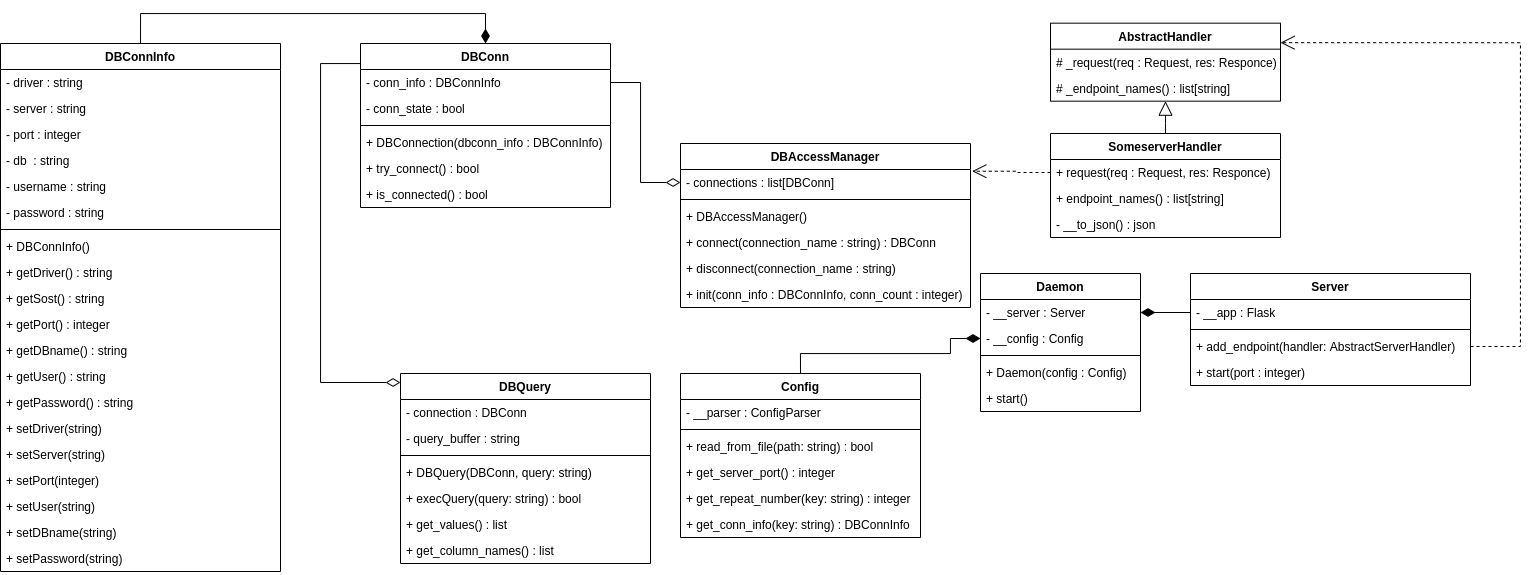
\includegraphics[width=16.5cm]{server_classes}}
	\caption{Диаграмма классов сервера.}
	\label{fig:server_classes}
\end{figure}

Пример реализации обработчика запросов (дочернего класса AbstractHandler) приведен в листинге \ref{auth_handler}. Класс AuthHandler обрабатывает запрос на авторизацию.

\begin{lstlisting}[label=auth_handler,caption=\text{AuthHandler.py.}]
from .abstract_handler import AbstractHandler
from database.dbconn import DBConn
from database.dbquery import DBQuery
from database.dbaccess_manager import access_manager
from server.key_data_checker import valid_key_checker
import json
import uuid
	
class AuthHandler(AbstractHandler):
	def request(self, req, res):
		res.content_type = "Application/Json"
	
		try:
			auth_data = json.loads(req.data)
		except json.decoder.JSONDecodeError:
			res.status_code=403
			res.data = json.dumps({"error" : "Empty fields"})
			return

		if not auth_data.__contains__('login')  or \
			not auth_data.__contains__('password'):
			res.status_code=403
			res.data = json.dumps({"error" : "Expected values was not received"})
			return
	
		state, data = self.__query_staff_data_from_db(auth_data['login'], auth_data['password'])
		if (not state):
			res.status_code=403
			res.data = json.dumps({"error" : "invalid fields"})
			return

		key = str(uuid.uuid4())
		data["password"] = key
		staff_id=data["employee"]["staff_id"]

		state, schedule = self.__query_staff_schedule(staff_id)
		if (not state):
			res.status_code=500
			return

		data["employee"]["schedule"] = schedule

		json_data = json.dumps(data)
		valid_key_checker.register_key(key, staff_id)

		res.data = json_data

	def __to_json_schedule(self, rows, column_names):
		arr = []
		l = len(column_names)
		for i in rows:
			d = {}
			d[column_names[0]] = str(i[0])
			for j in range (2, l):
				d[column_names[j]] = str(i[j])
			arr.append(d)
		return arr
	
	def __to_json_staff_schedule(self, rows, column_names):
		out_json_obj = {}
		row = rows[0]
		for access in range(0, 2):
			out_json_obj[column_names[access]] = str(row[access])
		
		passport_json={}
		for ps in range(11, len(row)):
			passport_json[column_names[ps]] = str(row[ps])

		positions_json={}
		for pos in range(8,11):
				positions_json[column_names[pos]] = str(row[pos])
	
		staff_json={}
		for staff in range(2, 8):
			staff_json[column_names[staff]] = str(row[staff])
			
		staff_json["passport"] = passport_json
		staff_json["position"] = positions_json
		out_json_obj["employee"] = staff_json
		return out_json_obj
	
	def __query_staff_schedule(self, uid):
		conn_name = str(uuid.uuid4())
		conn = access_manager.connect(conn_name)
	
		str_query = \
			"""SELECT * FROM schedule WHERE employee_id={}""".format(uid)
		query = DBQuery(conn, str_query)
		if not query.execQuery():
			return False, None
		else:
			schedule = query.get_values()
		access_manager.disconnect(conn_name)
		return True, self.__to_json_schedule(schedule, query.get_column_names())	
	
	def __query_staff_data_from_db(self, login, passw):
		conn_name = str(uuid.uuid4())
		conn = access_manager.connect(conn_name)
		str_query = \
			"""SELECT a.login, a.access_level, s.*, p.*, ps.* 
				FROM staff s LEFT JOIN access a ON s.staff_id=a.employee 
					JOIN position p ON position=p.pos_id 
					JOIN passports ps ON s.passport=ps.pass_id 
						WHERE a.login='{}' AND a.password='{}';""".format(login, passw)
		query = DBQuery(conn, str_query)
		if not query.execQuery():
			return False, None
		else:
			result = query.get_values()
	
		if len(result) == 0:
			return False, None
	
		access_manager.disconnect(conn_name)
		return True, self.__to_json_staff_schedule(result, query.get_column_names())	
\end{lstlisting}

\subsection{Реализация клиентской части}

В приложении для хранения, сериализации и десериализации данных, хранящихся в базе данных, были реализованы специальные классы, наследующиеся от класса ISerializable (листинги \ref{ISerializable_h}). 

\begin{lstlisting}[label=ISerializable_h,caption=\text{ISerializable.h.}]
#pragma once

#include <QByteArray>
#include <QDebug>
	
template <typename T>
struct ISerializable
{
	virtual ~ISerializable() noexcept = default;
	virtual T serialize() const { qFatal("Use undefined function"); }
	virtual bool deserialize(const T&) noexcept { qFatal("Use undefined function"); }
};	
\end{lstlisting}

Пример такого класса (для таблицы access) приведен в листингах \ref{access_data_h}-\ref{access_data_cpp}.

\begin{lstlisting}[label=access_data_h,caption=\text{access\_data.h.}]
	#pragma once

#include "QJsonHeaders.h"
#include "core/iserializable.h"
#include "types/staff.h"

class AccessLevel : public ISerializable<QJsonValue>
{
public:
	enum class AccessLevelEnum
	{
		Admin,
		Main,
		Registry,
		Vet
	};

	virtual bool deserialize(const QJsonValue &value) noexcept override;
	virtual QJsonValue serialize() const override;
	QString toString();

private:
	AccessLevelEnum current;
};

class AccessData final : public ISerializable<QJsonObject>
{
public:
	virtual bool deserialize(const QJsonObject &) noexcept override;
	virtual QJsonObject serialize() const override;

	QString getLogin() const;
	uint64_t getUid() const;
	QByteArray getPassword() const;
	AccessLevel getLevel() const;
	const Staff &getOwner() const;
	void setLogin(const QString &value);
	void setPassword(const QByteArray &value);
	void setLevel(const AccessLevel &value);
	void setOwner(const Staff &value);

private:
	uint64_t uid;
	QString login;
	QByteArray password;
	AccessLevel level;
	Staff employee;
};
\end{lstlisting}

\begin{lstlisting}[label=access_data_cpp,caption=\text{access\_data.cpp.}]
#include <QVariant>

#include "user_data.h"
#include "json_fields.h"

bool AccessLevel::deserialize(const QJsonValue & v) noexcept
{
	QString value = v.toString();
	bool is_ok = false;
	if (value == AccessLevelType::access_vet)
	{
		current = AccessLevelEnum::Vet;
		is_ok = true;
	}
	else if (value == AccessLevelType::access_main)
	{
		current = AccessLevelEnum::Main;
		is_ok = true;
	}
	else if (value == AccessLevelType::access_admin)
	{
		current = AccessLevelEnum::Admin;
		is_ok = true;
	}
	else if (value == AccessLevelType::access_registry)
	{
		current = AccessLevelEnum::Registry;
		is_ok = true;
	}

	return is_ok;
}

QJsonValue AccessLevel::serialize() const
{
	QJsonValue value;
	switch (current)
	{
		case AccessLevelEnum::Vet:
			value = QJsonValue(AccessLevelType::access_vet);
			break;
		case AccessLevelEnum::Main:
			value = QJsonValue(AccessLevelType::access_main);
			break;
		case AccessLevelEnum::Admin:
			value = QJsonValue(AccessLevelType::access_admin);
			break;
		case AccessLevelEnum::Registry:
			value = QJsonValue(AccessLevelType::access_registry);
			break;
	}

	return value;
}

QString AccessLevel::toString()
{
	QString value;
	switch (current)
	{
		case AccessLevelEnum::Vet:
			value = AccessLevelType::access_vet;
			break;
		case AccessLevelEnum::Main:
			value = AccessLevelType::access_main;
			break;
		case AccessLevelEnum::Admin:
			value = AccessLevelType::access_admin;
			break;
		case AccessLevelEnum::Registry:
			value = AccessLevelType::access_registry;
			break;
	}
	return value;
}

bool AccessData::deserialize(const QJsonObject &document) noexcept
{
	bool ok = true;
	uid = document.value(AccessJson::field_acc_id).toVariant().toULongLong(&ok);
	login = document.value(AccessJson::field_acc_login).toString();
	password = document.value(AccessJson::field_acc_password).toVariant().toByteArray();
	ok &= employee.deserialize(document.value(AccessJson::field_acc_employee).toObject());
	ok &= level.deserialize(document.value(AccessJson::field_acc_access_level));
	return ok;
}

QJsonObject AccessData::serialize() const
{
	QJsonObject root;
	root.insert(AccessJson::field_acc_id, QJsonValue::fromVariant(QVariant::fromValue(uid)));
	root.insert(AccessJson::field_acc_employee, employee.serialize());
	root.insert(AccessJson::field_acc_login, login);
	root.insert(AccessJson::field_acc_password, QJsonValue::fromVariant(password));
	root.insert(AccessJson::field_acc_access_level, level.serialize());
	return root;
}

QString AccessData::getLogin() const
{
	return login;
}

void AccessData::setLogin(const QString &value)
{
	login = value;
}

uint64_t AccessData::getUid() const
{
	return uid;
}

QByteArray AccessData::getPassword() const
{
	return password;
}

void AccessData::setPassword(const QByteArray &value)
{
	password = value;
}

AccessLevel AccessData::getLevel() const
{
	return level;
}

void AccessData::setLevel(const AccessLevel &value)
{
	level = value;
}

const Staff& AccessData::getOwner() const
{
	return employee;
}

void AccessData::setOwner(const Staff &value)
{
	employee = value;
}
\end{lstlisting}

\subsection{Примеры работы программы}

Рассмотрим некоторые примеры работы программы и ее интерфейсы.

На рисунке \ref{fig:auth} представлено окно авторизации.

\begin{figure}[!h]
	\center{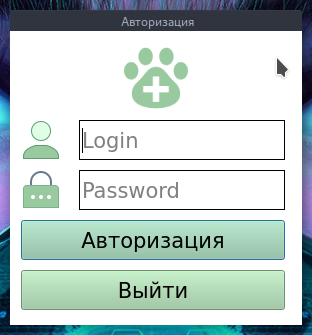
\includegraphics[width=6cm]{auth}}
	\caption{Окно авторизации.}
	\label{fig:auth}
\end{figure}

\newpage
На рисунке \ref{fig:admin} представлен профиль администратора. На рисунке \ref{fig:acc_info} представлена вкладка и ифнормацией об аккаунте.

\begin{figure}[!h]
	\center{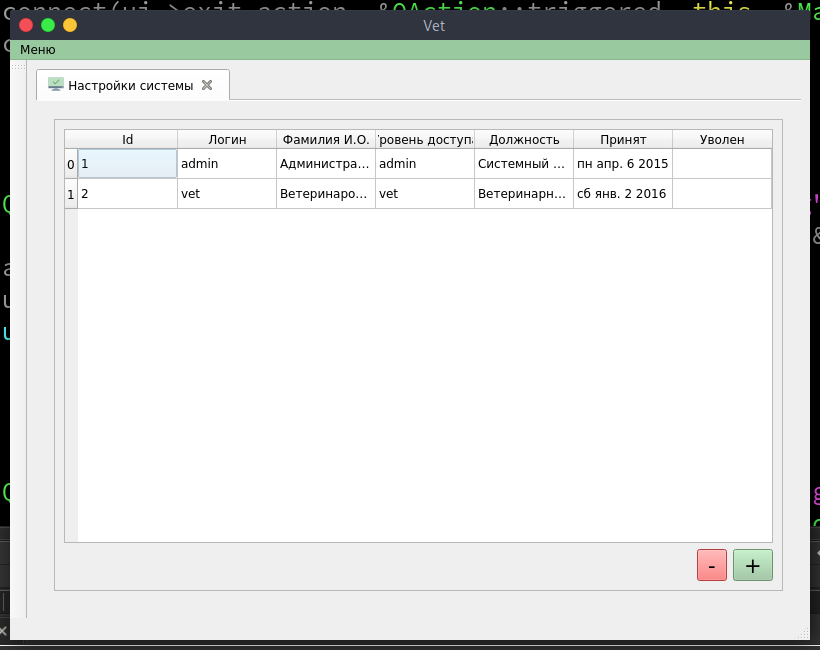
\includegraphics[width=13cm]{admin}}
	\caption{Профиль <<администратор>>.}
	\label{fig:admin}
\end{figure}

\begin{figure}[!h]
	\center{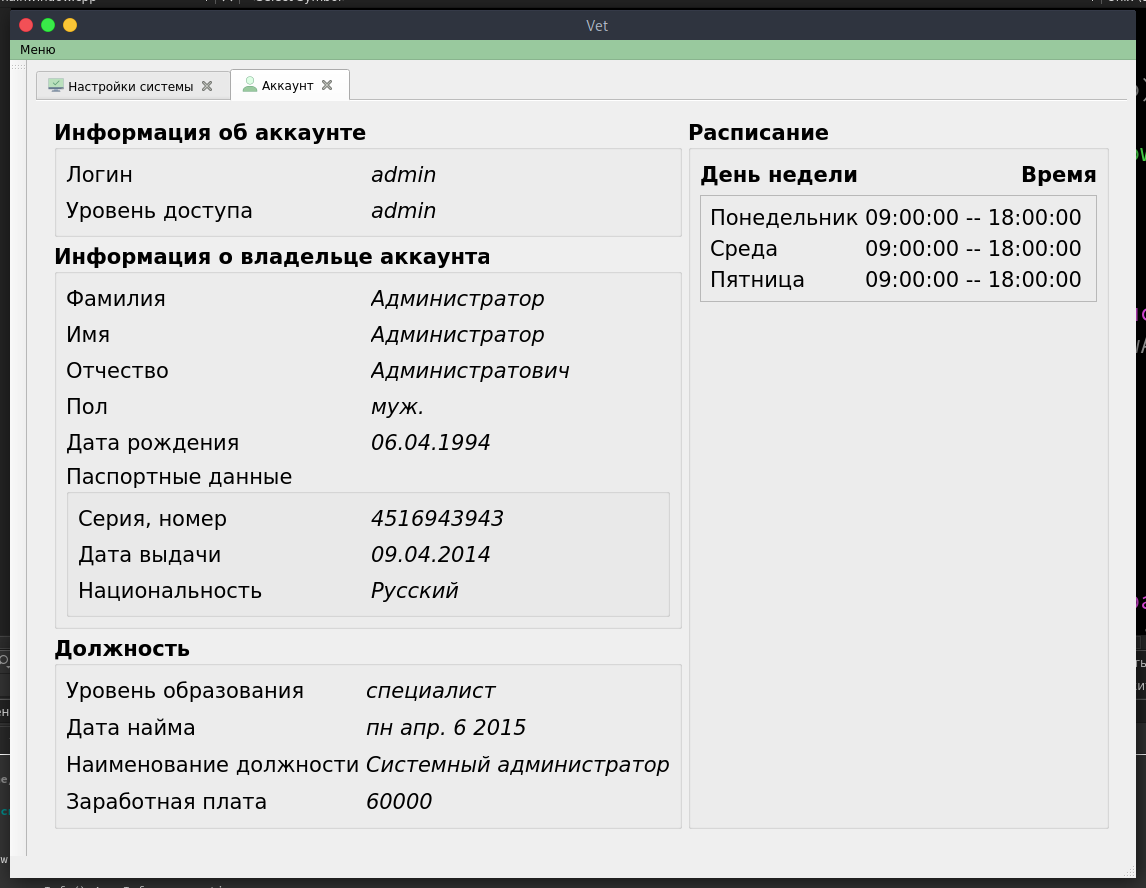
\includegraphics[width=13cm]{acc_info}}
	\caption{Информация об аккаунте.}
	\label{fig:acc_info}
\end{figure}

\newpage
На рисунке \ref{fig:vet} прелставлен профиль врача-ветеринара. На рисунке \ref{fig:visit} прелставлена форма заполнения нового осмотра ветеринара. На рисунке \ref{fig:prescr} прелставлена форма заполнения нового назначения.

\begin{figure}[!h]
	\center{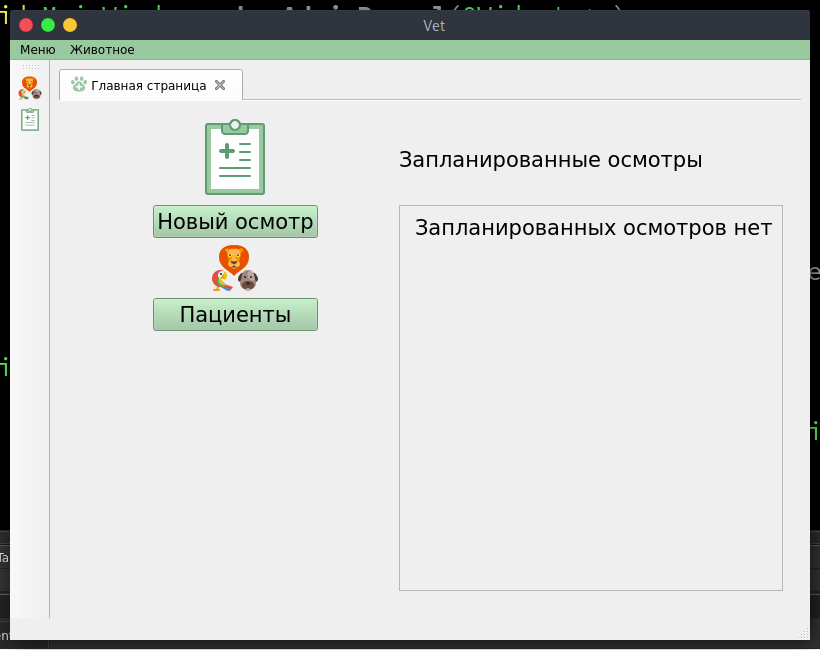
\includegraphics[width=13cm]{vet}}
	\caption{Профиль <<ветеринар>>.}
	\label{fig:vet}
\end{figure}

\begin{figure}[!h]
	\center{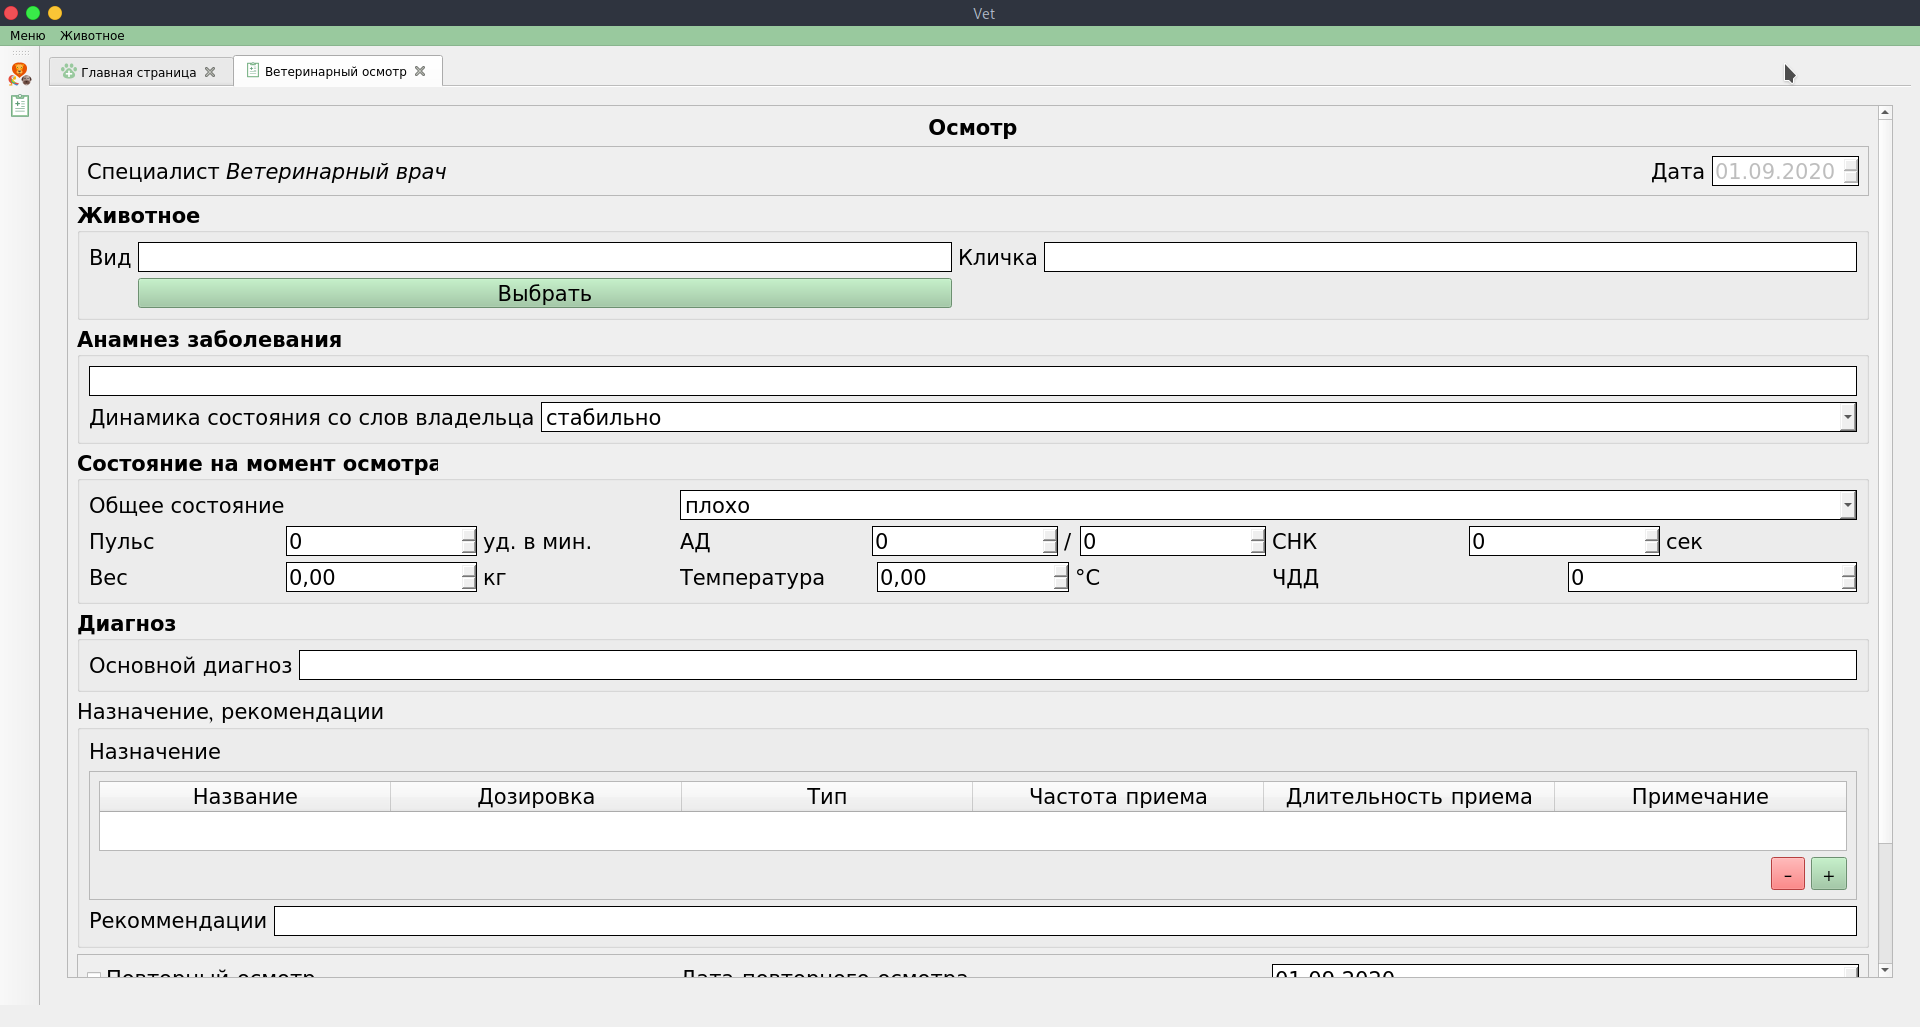
\includegraphics[width=16.5cm]{visit}}
	\caption{Новый осмотр.}
	\label{fig:visit}
\end{figure}

\newpage
\begin{figure}[!h]
	\center{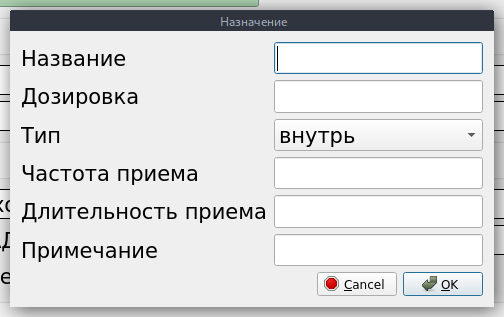
\includegraphics[width=14cm]{prescr}}
	\caption{Новое назначение.}
	\label{fig:prescr}
\end{figure}

\textbf{Выводы из технологического раздела}

Таким образом, в данном разделе были выбраны средства реализации проекта, приведены листинги и показаны примеры работы программы.

\newpage
\section*{Заключение}
\addcontentsline{toc}{section}{Заключение}

В ходе данной работы было реализована информационная система ветеринарной клиники, предназначенная для сбора, обработки, хранения и выдачи информации и принятия управленческих решений.

В процессе работы были получены знания, касающиеся организации межсетевого взаимодействия, создания и настройки сервера,  а также закреплены навыки проектирования и реализации базы данных.

\newpage
\begin{thebibliography}{3}
\addcontentsline{toc}{section}{Список литературы}

\bibitem{interfax_14}
Число домашних животных в РФ выросло на 14\% за три года [Электронный ресурс]. -- Режим доступа: https://www.interfax.ru/russia/631927, свободный -- (07.07.2020).

\bibitem{karpova02}
Карпова, И. П. Базы данных. Учебное пособие. / И. П. Карпова. – М.: Московский государственный институт электроники и математики (Технический университет), 2009.

\bibitem{nosql}
Фулер, Мартин. NoSQL: новая методология разработки нереляционных баз данных. / Мартин Фулер, Прамодкумар Дж. Садаладж. Пер. с англ. – М. : ООО «И. Д. Вильямс», 2013. – 192 с.

\bibitem{Giznburg}
Гинзбург А. Г., Иванов А. Д., Организация ветеринарного дела, 2 изд., М., 1970.

\bibitem{Vetenz}
Ветеринарная энциклопедия, т. 1, М., 1968.

\bibitem{infect_viki}
Инфекционные заболевания [Электронный ресурс]. -- Режим доступа: https://en.wikipedia.org/wiki/Infection, свободный -- (07.07.2020).

\bibitem{protoz_viki}
Протозойные инфекции [Электронный ресурс]. -- Режим доступа: https://en.wikipedia.org/wiki/Protozoan\_infection, свободный -- (07.07.2020).

\bibitem{gelm_viki}
Гельминтозы [Электронный ресурс]. -- Режим доступа: https://en.wikipedia.org/wiki/Helminthiasis, свободный -- (07.07.2020).

\bibitem{viral_viki}
Вирусные заболевания [Электронный ресурс]. -- Режим доступа: https://en.wikipedia.org/wiki/Viral\_disease, свободный -- (07.07.2020).

\bibitem{goals}
Цели, задачи и предмет деятельности учреждений ветеринарии [Электронный ресурс]. -- Режим доступа: http://www.chelagro.ru/about/subordinated/goals\_and\_objectives\_of\_veterinary\_institutions.php, свободный -- (08.07.2020).

\bibitem{karpova}
Карпова, И. П. Введение в базы данных. Учебное пособие. / И. П. Карпова. – Спб.: Питер, 2020. – 240 с.

\bibitem{martin_arch}
Мартин, Р. Чистая архитектура. Искусство разработки программного обеспечения. / Р. Мартин. — СПб.: Питер, 2018. — 352 с.

\bibitem{rest_habr}
Архитектура REST. [Электронный ресурс]. -- Режим доступа: https://habr.com/ru/post/38730/, свободный -- (20.08.2020).

\end{thebibliography}

\end{document}